\chapter{The Greater Good}

\begin{wrapfigure}{O}{\figwidth}
	\begin{center}
		
\includegraphics[width=\figwidth]{pics/10/1.png}
	\end{center}
\end{wrapfigure}
Interrogator Greg Sargent was not having a good day, in fact, given that he was currently waist deep in a septic pipe, it's safe to say that he was having an incredibly shitty day. 
He'd spent his entire morning in meetings with the other Interrogators, his afternoon had been one long argument with the Inquisition's most tedious personnel officer, and then he'd been called away to deal with this mess. 
Now, instead of eating a well earned dinner, he was trying to pick his way through a rat's nest of trip wires while arguing philosophy and speculating how many showers he was going to need- all because his squad's demolitions expert had stopped taking his meds again.

Twitch wasn't having a good day either, he could hear the Orks moving through the pipes around him, but didn't have anything heavy enough to blast through to them. 
If Doc and Tink hadn't stolen his supplies when he'd told them about the Kommando raid Twitch could've easily wiped out the greenskins, instead he'd been reduced to trying to snipe them through the walls with his laspistol. 
To make matters worse, the traitorous bastard coming up the pipe was destroying the few perimeter defenses he'd been able to rig. 
Twitch stopped perforating the walls for a moment to shout down the pipe, reminding Sarge that he'd always said never to trust anyone over the rank of Sergeant.

Doc, Tink, and Nubby were having a great day. 
Tink had jacked a screen into the maintenance cameras and everyone was enjoying the show. 
They took turns critiquing Sarge's arguments about the nature of rank and Twitch's rebuttals. 
After the second time Sarge tripped into the muck Tink asked if this wasn't a bit much, especially coming from Doc. 
The medic held up his travel orders and pointed to the name of the vessel that'd be taking them to Tau space. 
With a grim smile Doc asked Tink if he'd ever heard the story about the time Nubby bought a warpship.

\greentext{>The All Guardsmen Party and the Greater Good}


\begin{wrapfigure}{O}{\figwidth}
	\begin{center}
		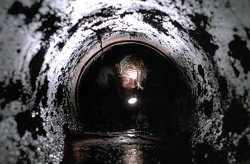
\includegraphics[width=\figwidth]{pics/10/2.png}
	\end{center}
\end{wrapfigure}
Eventually Sarge got Twitch out of there, it was a good show while it lasted though. 
The whole experience actually seemed to cheer him up, nothing like a slog through a river of shit and booby-traps to get a soldier back to their roots. 


The weeks before that had been rough on Sarge, he wasn't cut out for meetings or other bureaucratic bullshit. 
We'd all noticed that he kept disappearing and was getting grumpier than usual, but put it down to him getting married or contracting some horrible disease. 
It wasn't until we were all given sets of honest-to-god deployment orders that we found out that the man had let himself get promoted. 
That was a nasty shock, it was like finding out the the regimental chaplain had sworn his soul to chaos.

Well actually no one but Twitch really took it that hard; 
there was a little moping and a lot of bitching, but eventually we came to terms with the situation. 
It's not like we didn't already follow his orders, the only difference now was that he was going to be busy running the whole team instead of focusing on keeping us alive. 
In a skewed way he was doing it for us, it was the only way we'd stop getting handed incompetent superiors to baby-sit. 
Still, Sarge had hid it from us and the first mission he'd landed us was ridiculous; 
the score had to be evened before things could return to normal, hence Twitch's little adventure.

Once Sarge and Twitch were hosed down everyone pulled together to help Sarge prep for the mission. 
Which is to say Doc helped and everyone else stayed out of trouble or annoyed people that were giving Sarge grief. 
It's amazing what people will agree to to get Nubby or Twitch to leave their office.

\begin{wrapfigure}{O}{\figwidth}
	\begin{center}
		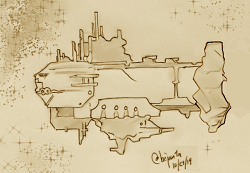
\includegraphics[width=\figwidth]{pics/10/3.png}
	\end{center}
\end{wrapfigure}
This time the mission wasn't a random investigation into something Oak's boys had dug up, it was a continuation of our previous one. 
The boss-man was very interested in the group of traitors we'd stumbled over and half-murdered in our escape from the Rogue Trader. 
He was of the opinion that they were responsible for most of the desertion problem and thought they'd been transporting the deserters off planet for some nefarious purpose. 
It was our job to track them down, figure out what was going on, then kill everyone for good measure. 
The problem was that the traitors and the trader had all buggered off after Bane blew up their base.

Our only real lead was the cloaked figure that had been bossing the traitors around. 
Oak's analysts had decided it was a Tau, a type of xenos that was fond of tech-heresy and corrupting the minds of honest imperial citizens. 
Since no one had seen the traitors or a massive army of deserters anywhere nearby the boffins thought that everyone must have fled to the region of space where the Tau lived, so the first step in finding them was going to be travelling halfway across the bloody galaxy to Tau space.

Of course the logistics of getting our squad all the way to Tau space were rather complex. 
It was too far to hitch a ride on navy vessels and if Oak was going to go through the trouble to send us down there he might as well send a few other teams to do inquisitive stuff. 
So instead of hiring a merchant vessel the Inquisitor decided to send one of his own ships, which was the real reason we weren't happy about the mission. 
Our squad was in for a several month trip on Oak's most recent acquisition, a freshly refurbished merchant ship known as the Occurrence Border.

This did not thrill us.

\begin{wrapfigure}{O}{\figwidth}
	\begin{center}
		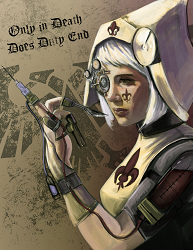
\includegraphics[width=\figwidth]{pics/10/4.png}
	\end{center}
\end{wrapfigure}
Despite the fact that we'd be travelling on a ship that had more in common with a warp-tainted space hulk than a proper vessel there were upsides to this arrangement: 
between the large number of teams being sent and the support staff that'd be staying on the ship, there were a lot of familiar names on the roster. 
Most of the survivors from the regiment were spread between the other teams, several of the cogboys and adepts we'd worked with were coming along, and Sarge got to help pick the ship's medical staff so a certain hospitaller was brought. 
The downside of this was that Doc began bouncing between being annoyingly cheerful and annoyingly worried. 
It depended on whether he was focusing on the fact that his girlfriend was coming along or the fact that his girlfriend might be eaten by daemons with the rest of us.

Doc's annoying tendencies aside, the final preparations went smoothly and everyone began transferring over to the Occurrence Border. 
We first met the rest of our team on the shuttle, Sarge had picked them all out beforehand, but Oak didn't like people talking about their orders before they left his ship. 


It had been obvious this mission was going to involve a lot more thinking and talking than any of us liked to do, so Sarge and Doc had mostly picked nerds to come with us. 
On the thinky side we had a xenos expert and a cogitator boffin. 
For the talky stuff we had an aging diplomat and a sneaky bugger who was supposed to be good at impersonating people. 
The final spot was filled by Fumbles, because the other Interrogators kept telling Sarge he should have a psyker and he was the least offensive one around.

Introductions were made, briefings were handed out, and most of the trip was spent explaining the odder aspects of the team to the newcomers. 
To their credit, they didn't start looking uneasy until the explanation reached Twitch's habits and why it was important to be nice to Fumbles.

\begin{wrapfigure}{O}{\figwidth}
	\begin{center}
		
\includegraphics[width=\figwidth]{pics/10/5.png}
	\end{center}
\end{wrapfigure}
There was a small welcoming party waiting for us when Sarge led us off the shuttle. 
A harassed-looking senior officer welcomed us aboard, then dumped our party onto a nervous looking midshipman and some crewmen. 
The poor middie apparently had a routine he was supposed to go through with new arrivals, unfortunately the first step was to have everyone's gear shipped ahead to their quarters by cargo servitors. 
Given our previous experiences with servitors on that ship, this didn't go over well with any of us. 
Twitch was of the opinion that we should kill the servitors immediately, just to be on the safe side.

Doc got Twitch to calm down and put his lasgun away while Sarge explained that, for personal reasons, we'd be carrying our own gear. 
The terrified midshipman didn't press the issue and skipped ahead to the orientation tour. 
While none of us really needed the tour, it was pretty fun, especially since our tour guide didn't know we'd been on the ship before.

The Occurrence Border was definitely in better condition than the last time we'd seen it, which really isn't saying much. 
The refit hadn't done anything about it's maze-like corridors or bizarre layout, but all the blood and battle damage had been cleared up, the gravity almost always went in the same direction, and none of the doors led to rooms full of daemonic fire. 
The biggest change we noticed was that the thousands of little notes had either been removed or replaced with official looking plaques that said the same thing, and there were maps at almost every junction. 
All-in-all the ship was in pretty good shape, though we did notice that certain sections on the maps were labeled "warp contaminated, do not enter" and every map had the comm code for the ship's Confessor printed under it.

\begin{wrapfigure}{O}{\figwidth}
	\begin{center}
		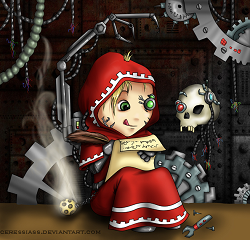
\includegraphics[width=\figwidth]{pics/10/6.png}
	\end{center}
\end{wrapfigure}
The high point of the whole tour was when a few of our pointed questions pushed the midshipman over the edge. 
He exploded into a passionate little tirade about how much effort had gone into refurbishing the ship and how poor its original condition was. 
Then he went on at great length about how badly the supply agent who'd purchased the ship had screwed up. 
Apparently the man had not only purchased a nearly derelict ship, he'd also managed to nearly lose it in the warp while transporting it to the shipyard. 
Given how much life and money had been lost in the deal, the incompetent had been lucky to only be re-assigned to one of Oak's "Suicide Squads". 
The kid couldn't figure out why Nubby looked so embarrassed and the rest of us kept cracking up.

Eventually we bullied the midshipman into taking us to engineering, where we traded him out for a more familiar guide. 
Jim the former tech-acolyte had been transferred to the ship a month ahead of us and was looking spiffy in his new Enginseer robes; 
it wasn't a surprise, Sarge had requested him and Hannah during the mission-prep. 


Everyone was happy to see Jim again, except for Tink who ignored the cogboy and wandered off to start poking at something expensive looking that was on a work-bench. 
Jim started bringing us up to speed on the ship's situation, pausing every few seconds to ask Tink to stop touching things. 
Before long a brief and ugly argument exploded between them, it ended with Sarge sending our techie to sit in the corner and try not to commit tech-heresy. 


Tink didn't respond well to the order, he grumpily demanded to know where Hannah was and asked if we could trade the "unscientific little zealot" for her. 
Everyone ignored him and Jim finished supplying us with all the information that the midshipman hadn't known or been willing to give us.

\begin{wrapfigure}{O}{\figwidth}
	\begin{center}
		
\includegraphics[width=\figwidth]{pics/10/7.png}
	\end{center}
\end{wrapfigure}
The half of our team that hadn't heard the story of our previous trip on the Occurrence Border had a little trouble following the discussion. 
They mostly just stood around and looked alternately confused and worried. 
Twitch and Nubby's explanations didn't help.

The main hydroponics bays were now midship and the tribals were their official caretakers. 
The psyker kids weren't with them anymore, they'd been claimed by Oak and were being raised into proper little team-killers. 
Also the bays were 99% krootoid-free.

Ol' Bill had been given a Juvenat treatment and was head of engineering. 
His surviving men had been given the treatment too and were bossing around a bunch of rather grumpy cogboys. 
Bill would have been there to greet us, but shuttle-bay 13C was stuck upside down and he was the only one who knew where its gravity controls were.

No more servitors had gone crazy since our adventure, but the crater the Cogtain had left at the bottom of the elevator to the bridge still glowed with daemonic light and screamed in binary at anyone who came near it. 
All attempts to patch it had failed, since it melted back to its original shape after a few hours. 
They'd just walled off the area and built a shrine to the emperor around it. 
It was probably completely safe.

All six "refurbished" Gellar field generators had been removed. 
They'd been replaced with a single brand-new big one and another big backup. 
Also: 
no, our official quarters were not near them and yes he and Hannah had cleared out a storage room across the hall from the main entrance. 
No one would complain if we set up camp there.

Finally, Jim supplied us with a far more accurate map of the ship than we'd originally been given. 
It had handy things labeled on it, like where the emergency food and weapon caches were and the location of everyone's quarters, including the medical team's. 
Doc took ownership of the map.

We bid Jim a fond farewell and headed for our conveniently empty store-room.

\begin{wrapfigure}{O}{\figwidth}
	\begin{center}
		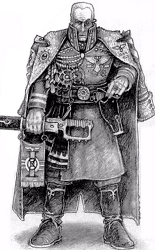
\includegraphics[width=\figwidth]{pics/10/8.png}
	\end{center}
\end{wrapfigure}
While we guardified our quarters a runner came for Sarge and directed him towards a pre-mission meeting. 
Since the rest of us had much more important things to do than slowly die of boredom, he wound up taking the three nerds and the infiltrator along. 
They hadn't been much help building barricades anyway.

The meeting consisted of half a dozen other full Interrogators and their minions, some of the ship's senior officers, a mechanicus magos, and the Captain. 
According to Sarge the Captain of the ship was either ex-navy or ex-administratum and didn't appear to be too happy with his assignment. 
He started things off by explaining that while he was not an Inquisitor or even an Interrogator, he was in charge of the ship and the only orders he'd be following were Oak's. 
It was his job to transport and supply everyone, regardless of whether their personal mission was recruitment, training, investigation, or archeotech hunting. 
Therefore his primary objective was to keep the Occurrence Border's cover, and hull, intact while making enough profit off trading to keep the ship running and everyone supplied. 
So unless everyone agreed that a certain mission needed to come first, he'd be choosing the ship's route and providing what resources he saw fit.

Being a military man, Sarge didn't see anything wrong with this, everyone else immediately started bickering of how important their missions were though. 
At first it was amusing to watch, especially since half the debaters refused to tell anyone else what their mission actually was, but after the second hour Sarge was ready to start shooting people. 
After sitting around and commiserating with the Captain and his officers for a while he just handed over a copy of our briefing and ditched the meeting. 
It wasn't like we even knew where in Tau space the deserters actually were yet.

\begin{wrapfigure}{O}{\figwidth}
	\begin{center}
		
\includegraphics[width=\figwidth]{pics/10/9.png}
	\end{center}
\end{wrapfigure}
The interrogators must have eventually reached a compromise, because a few hours after Sarge returned the vox system told everyone to prepare for warp and the Gellar Field Generator kicked on, nearly frying Twitch as he inspected it for bombs. 
We all grabbed our weapons, ignored the worried looks our teammates gave us, and prepared for the worst. 
It was sort of disappointing when nothing happened.

Over the first few days of the trip we built a nice miniature fire-base in our gellar-field adjacent room, but couldn't convince any of our teammates to move in. 
Even Fumbles bailed on us, he said the generator made his head hurt, and the rest of the crazy bastards seemed to think that rooms with real beds and bathrooms were better than being in the absolute least-warpy part of the ship. 
We didn't press the issue, it was their funeral.

Anyway after the base was up we didn't really know what to do with our time and the trip to Tau space was a damned long one. 
Sarge, being a rather cynical individual, imagined how the rest of us would keep ourselves entertained over a several month voyage and went to talk with the Captain. 
Before any of us could really start to enjoy our leisure time, much less cause serious trouble, a shipwide announcement was made. 


The gist of it was that "Heresy grows from idleness" and "Layabouts will not be tolerated". 
If anyone on the ship didn't have something to do to prepare for their mission they had three options: 
find a job on the ship, report to Sarge's new physical fitness class, or take a long walk out a short airlock. 
There was a short debate between us on which option was the least horrible, that is until Nubby verified that we wouldn't be given a voidsuit or let back inside the airlock after our "walk."

\begin{wrapfigure}{O}{\figwidth}
	\begin{center}
		
\includegraphics[width=\figwidth]{pics/10/10.png}
	\end{center}
\end{wrapfigure}
Doc wound up in the medbay where, to everyone else's amusement, he was put to work under his Hospitaller girlfriend. 
This arrangement led to numerous tasteless jokes. 
Anyway, despite what everyone imagined, Doc spent most of his time on his feet, dealing with the impressive number of injuries that the Occurrence Border caused on a daily basis.

Tink signed up for engineering where he managed to horribly insult or disgust, depending on gender, almost every tech-priest on the ship. 
After the fifth accusation of tech-heresy, not to mention the third harassment report, Sarge asked Ol' Bill for a favor. 
Tink was assigned as the aged engineer's personal assistant and was kept in line via regular percussive maintenance with a spanner.

Since mining the entire vessel was out of the question, Twitch took it upon himself to patrol the ship for kommandos and the like. 
Nubby, figuring this for a snipe-hunt and a great way to avoid strenuous exercise, joined him and dragged Fumbles along for moral support. 
He hadn't counted on the fact that significant portions of the ship were still warp-tainted and tended to manifest all sorts of warp-phenomena whenever the navigator hit a bump. 
The three of them got far more of the "Occurrence Border experience" than the rest of us, frequently finding themselves working with the ship's armsmen, clerics, and engineers to beat back minor daemons and seal holes in reality. 


The trio's adventures were as numerous as they were unbelievable. 
Every night Nubby would regale us with tales of derring-do and personally claimed no less than three bloodthirster kills before the trip ended. 
Fumbles happily basked in the dubious glory of these stories and Twitch was, well, Twitch. 
One night, while drinking, he quietly told us that when the turbulence was bad random doors opening to rooms of fire were still a thing, also the mysterious poker room now had a fighting ring occupied by a chainsword wielding skeleton. 
The skeleton had waved at him.

\begin{wrapfigure}{O}{\figwidth}
	\begin{center}
		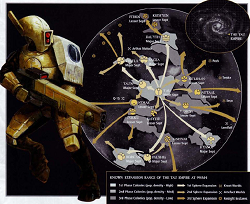
\includegraphics[width=\figwidth]{pics/10/11.png}
	\end{center}
\end{wrapfigure}
After we settled into our roles the long trip went by without any incidents. 
Well, at least without any major incidents. 
Actually, let's just say that no one died horribly. 
Almost no one. 
Well, no one who's name we actually remembered. 
The important thing is that everyone on OUR team was alive and functionally sane when we reached the edge of Tau space.

The adepts and the infiltrator had spent the whole trip going through the he data that Oak gave us and what came in via astropath. 
As far as we could tell the only thing they'd established with all that work was that the deserters had left the Imperium from the top-leftish direction on the map. 
This didn't overly impress us, but it was enough information for the Captain to plan his route and as we got closer to the border some useful data began to come in.

Apparently this section of space was lousy with Ordos Xenos agents keeping an eye on the Tau. 
Every time we stopped to refuel or do a little trading the adepts would send out queries and they slowly narrowed down our destination to a cluster of what the nerds called "buffer systems." 

According to the diplomat and xenos expert the border between the Imperium and the Tau empire were a little fuzzy out here. 
The big, important systems all had clear owners, but there were a large number of more marginal worlds that were more or less independent. 
The adepts explained how they served an important purpose involving trade and tension and other stuff, but Doc was the only one who even tried to follow it all. 
As far as we were concerned we were headed towards a bunch of worlds that were half human and half xenos because they were too shit for either side to care about.

After a few stops to drop off other teams and pick up cargo the Captain steered us towards the cluster and Sarge was forced to pick a world to start the mission on. 
In the end he ignored all the data and estimates provided by the adepts and just chose the only one with a permanent agent on it.

\begin{wrapfigure}{O}{\figwidth}
	\begin{center}
		
\includegraphics[width=\figwidth]{pics/10/12.png}
	\end{center}
\end{wrapfigure}
The Occurrence Border came out of warp at our destination with the usual groans, clangs, and small explosions and we made our final preparations for the mission. 
Nubby grudgingly supplied the rest of the team with weapons, Tink grabbed all the gadgets he could carry from the engineering department's stores, Twitch repacked most of his traps, and Doc annoyed everyone with his melodramatic goodbyes. 
After Sarge handed command of his PT class over to the ship's bosun he corralled everyone into the shuttle-bay for a final briefing.

To our surprise the Captain actually came down to see us off. 
He and Sarge had gotten along rather well and the Captain personally handed over the ship's contact codes and the briefcase of local currency that would act as our budget. 
Sarge saluted the man and promised to meet him for drinks when the Occurrence Border came back through the cluster in three months, then led us onto the shuttle that would take us to the planet.

As we flew down the xenos expert and diplomat tried their best to remind us how things worked on this world. 
They managed to fit an entire crash course on the socio-political situation, the cultural and economic status of the cluster, and the history of the Tau Empire into a two hour shuttle trip. 
None of us really listened though, we knew that "border world" meant a barely colonized wilderness, possibly with a few xenos that no one had gotten around to killing yet.

The spaceport we landed in wasn't the biggest we'd seen, but it was definitely the cleanest. 
Several teams of men came out and started unloading our shuttle, and one of them discretely led us through into a service tunnel. 
A bit of walking and a short drive later we found ourselves standing on a street-corner in the oddest looking city any of us had ever seen. 
As a mixed crowd of humans and xenos parted around us Nubby quietly asked the adepts if they'd mind giving that lecture again.

\begin{wrapfigure}{O}{\figwidth}
	\begin{center}
		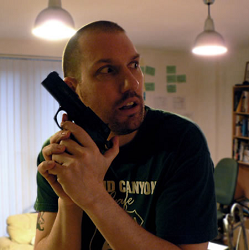
\includegraphics[width=\figwidth]{pics/10/13.png}
	\end{center}
\end{wrapfigure}
Just saying that place was weird doesn't even begin to cover it. 
It might have been easier to handle if it was just a xenos city, but the way humans and familiar pieces of imperial architecture were mixed in was just uncanny. 
The crowds of people heading to work looked normal at first, then you realised half of them were fricken blue. 
You'd see a shrine to the Emperor, with all the nice, normal arches and skulls and everything, then right next to it would be a giant mushroom-looking building and no-one even seemed to notice. 
On top of that all the humans looked subtly wrong, it wasn't their clothes or hairstyles, it was they way they walked and talked. 
While we all stared and tried to figure out what was going on, Fumbles put his finger on it: 
everyone around us was… happy, or at least not as wearily miserable as normal workers should be. 
It was damned unsettling.

Twitch and Tink both went into a sort of overload caused by the sheer number of xenos surrounding us and the amazing array of tech being used in the city respectively. 
Both had to be restrained while Sarge and the adepts negotiated a vehicle rental, and the struggle attracted quite a bit of attention. 
Luckily none of us were in uniform or obviously armed, so Doc and the infiltrator were able to convince all the curious onlookers that everything was fine and no-one was about to start a shooting spree.

When Sarge returned with the vehicle (a normal ground truck, thank the Emperor, Tink would've exploded if it had been one of the hovering xenos ones), we piled in and drove towards our local contact's address as fast as possible. 
We got about half a klick before we heard a siren and our truck suddenly slowed down and pulled over while Tink struggled with the wheel and swore at it. 
Nubby just barely stopped Twitch from snap-shotting the Tau police officer who wanted to know what the hurry was and where the hell we'd learned to drive.

\begin{wrapfigure}{O}{\figwidth}
	\begin{center}
		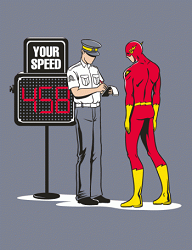
\includegraphics[width=\figwidth]{pics/10/14.png}
	\end{center}
\end{wrapfigure}
So no shit, there we were, a highly trained and heavily armed Inquisitorial goon squad, chasing a bunch of traitorous deserters on an alien world, and we'd just been pulled over for speeding. 
Not our best moment.

Mortified doesn't even begin to cover it. 
Almost everyone just sort of sat there and stared ahead, thinking about how our cover was going to be blown and how the entire local government would come down on us, all because of a damned speeding ticket. 
The only sounds were Tink's muttered curses as he tried to figure out what had forced the truck to stop, Doc's prayers, and our social infiltrator fast-talking the officer. 


Thank the Emperor for that sneaky bastard and his bull-shitting skills. 
Through impressive series of lies, excuses, distractions, and a little bribery he managed to hide the fact that we didn't have any sort of identification and even managed to talk some directions out of the cop too. 
Despite how well things worked out though, it was a sobering and educational experience which really drove in how far we were from home. 
On an Imperial world the local police tended to ignore anything less than an outright murder by a man in a Guard uniform. 
Hell, no one even blinked at one of us carrying a lasgun around. 
It seemed they were a lot less accommodating around here.

As the officer walked away Sarge began to worry. 
Given that we'd nearly gotten into a life and death struggle with the authorities while leaving the shuttleport, his first mission as Interrogator seemed doomed to failure before the end of the month. 
His mood was not improved when Tink ripped out the pesky little thingy that had forced us to pull over, causing the police officer turned around and walk back. 
While the infiltrator hastily tried to explain why we'd just ripped out our vehicle's government-mandated Identification and Emergency Control Device, Sarge decided we'd be lucky to make it to the end of the week.

\begin{wrapfigure}{O}{\figwidth}
	\begin{center}
		
\includegraphics[width=\figwidth]{pics/10/15.png}
	\end{center}
\end{wrapfigure}
Eventually we managed to sort things out and reached the address we'd been given for our local contact. 
It turned out to be a large, official-looking building in Imperial style, but built out of the weird tan stuff the Tau liked to use. 
In a fit of sanity we all decided that trooping in the front door of a government building and knocking on the Secret Inquisitorial Agent's door would be a stupid thing to do, so our xenos and cogitator experts were sent to figure out how to use one of the public comm terminals to call him. 
Tink complained that he wasn't sent too, but didn't get any sympathy.A few minutes later the adepts came back and directed us around to an unmarked passage which took us deep into the building.

The passage ended at an impressive security door which opened into a surprisingly posh office and sealed seamlessly into the wall behind us. 
A large, slightly overweight man sat at a desk with a nameplate which declared him to be "General Weebu, Head of Interplanetary Security." There was a brief moment of panic as all of us took in the title and realized we'd just walked, nearly unarmed, into the planet's intelligence headquarters, then the man stood up and extended his hand to Sarge. 
In a booming voice he introduced himself as Lars Weebu, Inquisitor of the Ordo Xenos, Retired.

Several questions flashed across our minds as we processed what we'd just seen and heard, such as if Inquisitors could really retire and how he'd wound up here. 
Unfortunately the first person to open their mouth was Nubby, who loudly asked why the Inquisitor was wearing a dress. 
A sort of congealed silence followed that remark, then Tink pointed out that it was more of a robe and lots of men wore robes. 
Nubby riposted by pointing out that "it's got flowers on, it's not a robe if it's got flowers on" and Tink conceded the point, but suggested they shouldn't judge him for his choice of clothing, the xenos had probably done something to his brain.

\begin{wrapfigure}{O}{\figwidth}
	\begin{center}
		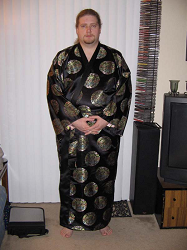
\includegraphics[width=\figwidth]{pics/10/16.png}
	\end{center}
\end{wrapfigure}
Nubby was the lucky one, he only got slapped upside the head by Doc, Tink got hit by Sarge. 
That was probably the third most embarrassing experience in Sarge's life, coming in above the speeding ticket, but below the apology he'd had to make for our trainees back when we were instructors for Oak. 
Face glowing, Sarge stepped over Tink's groaning body and did his best to explain that, while all of his team members were excellent soldiers, some had suffered mental damage in their battles. 
The ex-Inquisitor stood there and looked stuffed for a few more seconds then muttered something about falling standards. 
He turned to face Nubby, who paled and tried to smile, then spent an inordinately long time explaining the cultural significance of Tau formal robes.

Now when I say inordinately long, I really mean it. 
The man just kept talking and talking, it wasn't until Sarge pointed out that "we" didn't want to take up his entire day that he wound down enough for us to get in our questions. 
Of course those questions immediately set him off again, we had to endure this whole rambling lecture about how after a century of fighting them he'd discovered how unique and vibrant Tau culture and society were. 


According to Weebu it was his duty, for the good of the galaxy as a whole, to preserve what aspects of it he could and incorporate them into the Imperium before their self destructive government doomed them all by provoking us. 
He'd worked to get this position so he could steer these free border worlds towards a brighter future; 
if only everyone could see than an alliance was possible and the benefit of sharing technology we could- blah, blah, blah, I'm a xenos loving weirdo. 
Sarge eventually had to stop him again when he started telling us about how many times the metal in an Honour Blade was folded.

\begin{wrapfigure}{O}{\figwidth}
	\begin{center}
		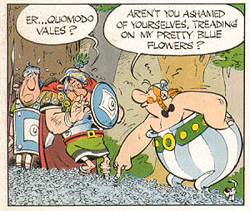
\includegraphics[width=\figwidth]{pics/10/17.png}
	\end{center}
\end{wrapfigure}
To say we were dubious about the ex-Inquisitor's sanity and loyalty is one hell of an understatement, especially since he never exactly said how he became an ex-Inquisitor, but he really was the only lead we had out here. 
When he could get a word in edgewise Sarge explained we were here to hunt down a large number of Guard deserters, their rogue trader transport, and the cloaked xenos who'd led them, then had the adepts fill in all the details they'd gathered. 
Weebu took this all in then directed us to sit and wait while he played with a xeno-cogitator thingy that popped out of his desk and made both Tink and the boffin drool.

As Weebu typed and read he gave us a quick rundown of the overall situation in the cluster. 
Almost every planet, or large station, was independently governed and worked with the rest of the cluster in a sort of defensive alliance. 
Some individual planets worked closely with the Tau government, others were more pro-Imperial, but as a whole the cluster wanted to stay a neutral buffer-state. 
They had a good thing going: 
everyone was making money off all the unofficial trade that went between the empires and no one's planet was being used as the arena for the latest Tau vs. 
Imperium pissing match.

Lately though, things were looking a little dicey. 
Someone with serious firepower was raiding stations and even a few planets in the cluster, completely destroying them and leaving no witnesses. 
Everyone was arming up and getting ready for a fight, but no one knew what the threat actually was and if their forces could take it. 
Some of the more pro-Imperial or pro-Tau planets were loudly saying that it'd better to lose their independence than be horribly murdered, while the rest waited to see if they could handle it themselves. 
So basically things weren't completely screwed up here, but a major incident could set off a serious shitstorm, or as Weebu put it: 
"Disturb the tranquility of my garden of tolerance." Weirdo.

\begin{wrapfigure}{O}{\figwidth}
	\begin{center}
		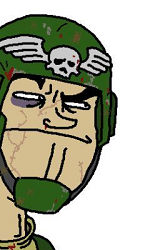
\includegraphics[width=\figwidth]{pics/10/18.png}
	\end{center}
\end{wrapfigure}
The whole point of the ex-Inquisitor's lecture was that it was not good time for a bunch of desperate, well-armed, military trained men to be wandering around the cluster looking for a little fun. 
And they definitely were wandering around the cluster, according to the reports he was looking at right then, every planet was seeing an influx. 
Unfortunately there weren't enough to account for the numbers we gave him, so it was probably just spillover from where the majority were heading. 
Therefore he would, both as a favor to us and for the good of his "garden," put his agents on tracking down those missing men.

Weebu suggested that we find ourselves a safehouse and brush up on the local culture and laws while he had an entire planet's spy agency do the legwork for us. 
Once his boys found the deserters he'd pass the info on and we could handle the messy parts while his agency kept its hands clean. 
This suited us nicely, but Sarge felt he should make at least a token effort and asked if there were any parts of the investigation we could help with. 


After a little thought the ex-Inquisitor reiterated his suggestion and added the local technology to the list. 
He cited a report that had just come in saying that several suspicious men had been pulled over for reckless driving, attempted to bribe the police officer, ripped out their vehicle's transponder, and attempted to bribe the officer again. 
These men were apparently so clueless that they hadn't even shielded their highly-illegal weapons from scanning or noticed the drones the officer had sent to tail their vehicle while he reported the incident. 
If it weren't for a highly placed official vouching for these men, they'd probably have been arrested by the SWAT team waiting and watching their truck right this second.

Sarge quietly agreed to Weebu's suggestion, then led us out the passage, cursing xenos, Tink, the Inquisition, deserters, Tink, smartasses, and Tink every step of the way.

\begin{wrapfigure}{O}{\figwidth}
	\begin{center}
		
\includegraphics[width=\figwidth]{pics/10/19.png}
	\end{center}
\end{wrapfigure}
The first order of business, after we verified that a SWAT team wasn't about to attack us, was to get a place to stay. 
Sarge dumped the problem on the adepts then grumpily ordered everyone else to sit in the truck and not touch anything. 
The three nerds did a lot of cogitator and comm work, then gave us a list of options and their prices. 
Doc wisely asked whether there were security deposits on these places and how likely random civilians were to walk into "the perimeter." With those thoughts in mind, Sarge vetoed every hab on the list, leaving us with a disused warehouse that, from the smell of it, had last been used to store live grox. 
That's the glamorous lifestyle of an Inquisitorial agent for you…

The next week, or whatever the hell you call seven 34 hour days, was spent doing exactly what the ex-Inquisitor had told us to. 
The cogitator boffin patched himself into the planet's network and pulled down a ludicrous amount of information. 
It was then crammed into our poor, overloaded brains by the other two adepts while Sarge walked back and forth behind us all, hitting anyone who wasn't paying enough attention. 
It was a fairly horrible experience, but it definitely worked. 
By the end we knew how the planetary governments worked, the basic functions of the local tech, and far, far too much about Tau formal robes. 
We all blamed Nubby for that last subject.

\begin{wrapfigure}{O}{\figwidth}
	\begin{center}
		
\includegraphics[width=\figwidth]{pics/10/20.png}
	\end{center}
\end{wrapfigure}
When word hadn't come from Weebu by the end of the week Sarge told us to keep ourselves busy by applying the knowledge that'd been crammed into us. 
He and Doc brushed up on the local lingo with the infiltrator and the adepts did some cogitator work, just in case Weebu wasn't actually going to get us the info we needed. 
Tink and Twitch worked on ways to evade the pesky weapons scanners and drones the locals used for security and Nubby took Fumbles to the park. 


The psyker had been having trouble with the alien minds around him, he could look into them, but couldn't really understand what he saw. 
At Nubby's suggestion he got some practical experience by sitting in the local park and invasively probing random xenos as they passed by. 
In retrospect this might have been highly unethical and dangerous, but no daemons were spawned during this practice and only two xenos suffered serious psychological damage, so we called it a success. 
Also Nubby came back with a fair bit of cash after these trips. 
We didn't ask how.

The start of our third week on the planet marked the end of Sarge's patience and a call was put into the ex-Inquisitor. 
None of us heard what the two men said to eachother, but after quite a long discussion Sarge came back and told us that we'd receive the information soon and there was even a way we could speed the process up: 
Weebu had two sources of information that he hadn't tapped yet for one reason or another, if we checked them out it'd save him some time and effort.

One lead was a moderately large bounty hunting organization operating out of a nearby city, the other was merchant shipping conglomerate. 
The bounty hunters had supposedly been grabbing a few of the deserters that had wound up on this planet and the merchants might have records of seeing the rogue trader's ship. 
We decided to visit the bounty hunters first, it was a shorter drive, and they were more our sort of people.

\begin{wrapfigure}{O}{\figwidth}
	\begin{center}
		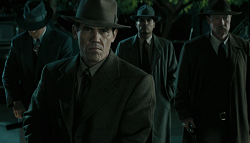
\includegraphics[width=\figwidth]{pics/10/21.png}
	\end{center}
\end{wrapfigure}
In retrospect Weebu had probably intended us to infiltrate the bounty hunters or tap their comms or something else sneaky, not kick down their door and demand to know "where the deserters at". 
That was his fault for not being specific though.

Well, we didn't actually kick any doors down and our grammar was a bit better than that, but that was the general theme of our investigation. 
Why bother prancing around to find out what they knew without them noticing? 
These were bounty hunters, they were one step above criminals and the only things they respected were money and violence, might as well talk to them in their own language. 
The only nod we made to subtlety was wearing the scan-proof trenchcoats Tink had spent so much time and money making. 
It was a very small nod too, more of a shrug actually, because the coats were mostly a way to conceal the fact that we were all armed to the teeth as opposed to hiding us. 
We figured that this planet's weapons laws were all well and good for public safety, but they really shouldn't apply to us.

We got a list of the hunters' main hangouts and watering holes, put the adepts in charge of watching the comm network for incoming trouble, then went out to be inquisitive. 
The plan was simple, the infiltrator would go in first with Fumbles and Twitch to scope the place. 
The second they pinpointed the boss or called for backup Sarge, Doc, and Nubby would come in and explain to everyone that the difference between a nice bar and a corpse-filled ruin was whether we left with the information we wanted. 
Tink would stay in the truck and be ready to drive us away if things got too hot.

Everyone whose opinion mattered thought this was an excellent plan, and we all congratulated Sarge on being the most tactically skilled Interrogator any of us had met.

\begin{wrapfigure}{O}{\figwidth}
	\begin{center}
		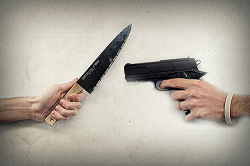
\includegraphics[width=\figwidth]{pics/10/22.png}
	\end{center}
\end{wrapfigure}
The first stop on our little information hunt was a rather shabby Tau building which was obviously the xenos equivalent of a shitty bar. 
Our advance party walked in and immediately picked out a big mother in xeno-armor and the slit-head he was arguing with as the guys in charge. 
Sarge got his game face on, stalked through the bar to the big guy, and demanded to know where the deserters were going. 
The big guy looked Sarge up and down, sneered, and told him to get lost, completely missing the fact that Nubby had circled behind him. 
Nubby's kick caught the bounty hunter in the groin and bent him double, Sarge's uppercut straightened him back out, and Doc's grab caught the Tau before he could leg it. 


The entire bar went quiet as the burly noncom turned to glower at the struggling xenos and repeated his question. 
The Tau shot a glance at the unconscious man on the bar, obviously decided the odds weren't in his favor, and babbled something none of us could quite understand. 
Sarge had to stand there and glower for a bit longer while the xeno-adept listening in translated for him, causing the alien to start shaking and babble a few more things, which in turn made the glowering last longer. 
Eventually the adept just told us the xenos knew nothing about deserters and suggest we let him go before he had the Tau equivalent of a heart attack.

Sarge picked the Tau up by the front of his armor, hefted him into the air with one hand, and tossed him over the bar. 
Doc quietly told the groaning xenos to stay down while Sarge announced that he'd be going through the entire bar until someone gave him an answer. 
Everyone thought this over, then a weasely looking man bolted for the exit while a few others drew shock-mauls. 


Twitch pegged the runner with a chair and the rising bounty hunters found themselves looking down the barrels of half a dozen laspistols. 
Nubby grinned evilly and asked everyone to line up single file and have their answers ready.

\begin{wrapfigure}{O}{\figwidth}
	\begin{center}
		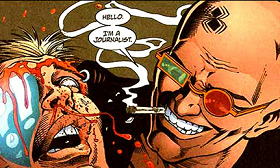
\includegraphics[width=\figwidth]{pics/10/23.png}
	\end{center}
\end{wrapfigure}
Ten minutes later we left the bar, secure in the knowledge that bounty hunters could listen to reason and that no-one there had known anything useful. 
Well no-one maybe the runner or the big guy had known something, but they hadn't woken up by the time we finished and we didn't feel like waiting: 
we still had a lot of other bounty hunters left to inquisit.

The second bar went a lot like the first, except this time Sarge just led with a sucker-punch on the meanest looking guy there instead of bothering to ask first. 
Once again there were a few slow learners, but a little violence got the point across before we had to kill anyone. 
Hell, we actually patched up the idiot who tried to stab Sarge in the back after we got the knife out of his hand and the table Sarge had nailed it to. 
All in all it was a very smooth operation and we even scored a few names.

Word of our little tour was apparently traveling ahead of us, because at the third and fourth stops they actually had someone waiting at the door with a list of everything they knew. 
It wasn't much more than the names we already had and directions towards where they might be found, but Fumbles said no one was lying so we bought everyone a round on the way out. 
It was sort of gratifying to have everyone bowing and scraping, being the big fish and not having to fight for everything is pretty nice. 


Shame the last group of bounty hunters weren't on the same page as the rest, but what can you expect from a bunch of feral xenos?

\begin{wrapfigure}{O}{\figwidth}
	\begin{center}
		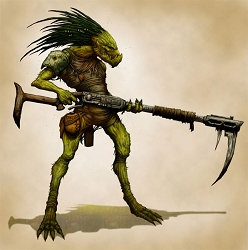
\includegraphics[width=\figwidth]{pics/10/24.png}
	\end{center}
\end{wrapfigure}
The last stop was the one everyone had been giving us directions towards, apparently it was where the big boys hung out. 
We pulled up to an odd Tau building which looked like a cross between a gambling den and a kennel and once again we found people waiting for us at the door. 
These guys weren't quivering in their boots like the rest had been, they were a pair of scarred brawler types and each was carrying a weird staff with hooked blades on the ends. 
They didn't try to keep us out, as we approached one of them came forward and said the boss was waiting to see us.

We accepted their invitation and entered the building through a hallway that had what we recognized as a weapons scanner in the middle. 
It was flanked by two Tau guards and a pair of ugly dog things with beaks, they looked a bit like the critters that infested the Occurrence Border's hydroponics bays. 
At Sarge's signal everyone slowly pulled out their laspistols and removed their power packs. 
The pistols were set in a bin near the scanner and the packs went into the outer pockets on our trenchcoats, then we all filed through the scanner. 
The scanner made a few quiet beeps and the hounds growled at us, but the guards waved us through. 
Fumbles casually tapped his combead twice and Sarge smiled to himself.

The room at the end of the hallway was dark, smoky, and smelled alien. 
A bunch of bounty hunters, mostly slit-heads, were lounging around some low tables with a few more of the hound things. 
It looked to be a total of fifteen potential hostiles plus three xenos we could barely make out in the far corner. 
All the humanoids had one of those spiky staves at hand, but Twitch and Fumbles said that they didn't see any guns. 
Not the best odds, but we'd survived far worse.

Sarge grimly led us to the xenos and found himself glowering upwards as they rose to their feet. 
All three were green, half a meter taller than Sarge, and looked exactly like the picture we'd seen in training labeled Kroot Carnivore.

\begin{wrapfigure}{O}{\figwidth}
	\begin{center}
		
\includegraphics[width=\figwidth]{pics/10/25.png}
	\end{center}
\end{wrapfigure}
So no shit, there we were, in the middle of a bounty hunter den, having a staring contest with three Kroot Carnivores, I think it surprised the hell out of them when none of us even flinched. 
They were probably used to people running for the exit when they all loomed over them like that, or at least taking a step backwards. 
Honestly though, these guys didn't impress us. 
We'd worked for, killed, and in one case eaten scarier things than a bunch of taller-than-average xenos. 
Hell, they didn't even make the top twenty… smelled horrible though.

Sarge matched their glares and asked if they were the ones capturing deserters. 
One of the Kroot let out a cackling laugh, and in terrible Low Gothic said they were and asked what we were going to do about it. 
It'd be cool to say Sarge and the xeno then exchanged some witty banter, trading threats and clues and all that. 
Unfortunately Sarge's Tau was about as bad as bad as the xenos' gothic, so most questions had to be repeated three or four times in both languages and eventually they just called over one of the human bounty hunters to act as a translator. 
Everyone kept glowering and talking in their most threatening voices though, nobody was going to let something as trivial as a massive language and cultural barrier get in the way of their intimidation attempt.

\begin{wrapfigure}{O}{\figwidth}
	\begin{center}
		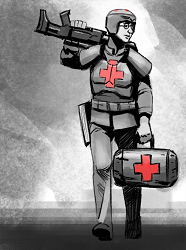
\includegraphics[width=\figwidth]{pics/10/26.png}
	\end{center}
\end{wrapfigure}
Once the translator was in place things started flowing a little more smoothly: 
everyone was able to question and threaten each other to their heart's content. 
Sarge asked who was paying the deserters' bounty, the Kroot on his right said it was someone on the neighboring pro-Tau world and asked if we'd like to meet him. 
Sarge asked why the bounty hunters would do that for us, prompting some more cackling laughter from Kroot and an assurance that their buyer was always in the market for more guardsmen, they'd even split the bounty with us if we came quietly.

While Sarge processed the threat Doc cut in, denying that we were guardsmen and explaining that we were fellow bounty hunters. 
After another bout of laughter the biggest xenos walked over to him and inhaled deeply. 
If we weren't guardsmen, he asked, why did we smell like lasguns, explosives, MREs, and paranoia. 
Doc fumbled for an answer and the Kroot went on to suggest that maybe he was mistaken about what those smells meant, maybe they meant we were a dance troupe, or a bunch of ecclesiarchs, or a the Inquisition.

In retrospect it was a joke, about on par with asking "who do you think you are, the bloody Inquisition?", but with the language barrier and everything else we didn't really get it. 
Everyone kept their poker faces though, except for Doc that is. 
Between the sinister laugh the Kroot have and the two and a half meter carnivorous alien towering over him, the medic interpreted this as an accusation and panicked.

This wasn't some raw recruit's panic though, he didn't scream "OH EMPEROR THEY'RE GOING TO KILL US" and run for the exit. 
Doc calmly, while holding eye contact with the Kroot, put his hands through the bottom-less side pockets in his trenchcoat, gripped the hot-shot lasgun slung across his chest, and blew the xenos in half.

\begin{wrapfigure}{O}{\figwidth}
	\begin{center}
		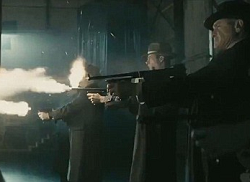
\includegraphics[width=\figwidth]{pics/10/27.png}
	\end{center}
\end{wrapfigure}
Doc's, er, outburst caught everyone but Twitch by just as much surprise as the bounty hunters, luckily they hadn't been expecting a fight or even thought we were armed. 
Three cheers for the primitive xenos notion of gun control, it made everything so much safer for those of us who ignored it.

Our little interview came to an end and the room practically exploded around us. 
Doc walked his fire over the second Kroot while Twitch, who'd been expecting this from the moment he entered the room, perforated the third. 
That wasn't quite enough to put them down, but they only managed a staggering pair of swipes that Sarge and Nubby both dodged before the second volley finished them. 
As the rest of the bounty hunters rose to their feet and seized their weapons all of us ruined the scan-proof coats Tink had made for us by hip-firing through them. 


The only reason it wasn't a complete slaughter was that a few of the smarter ones ran instead of trying to rush us. 
We gunned down the bird-dog things first, then shifted fire towards the stupider bounty hunters as they closed. 
Between four heavy lasguns, a pair of pistols, and Fumbles body-puppeting one of the few humans. 
none of them managed to lay a hand on us. 
Doc did catch a thrown beer bottle to the face though, but it missed his eyes and Nubby assured him his girlfriend wouldn't mind a few small facial scars.

While we all brought guns to a knife fight Tink got the truck's engine running and the cogitator adept commed us. 
He warned us that the police had dispatched a pair of cars to check out the noise and recommended getting the hell out of there. 
We were almost to the truck when the a police skimmer landed across the road from it and two officers, a tau and a human, stepped out of it and launched a pair of drones into the air.

Tink evaluated his chances of outrunning their flying car with his rental ground-truck, then poked his plasma gun out through the driver window and aimed it at the rear of their car.
\begin{wrapfigure}{O}{\figwidth}
	\begin{center}
		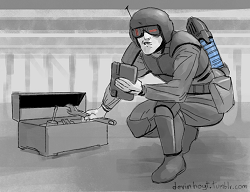
\includegraphics[width=\figwidth]{pics/10/28.png}
	\end{center}
\end{wrapfigure}
Now at this point we'd all been through a few lectures on Tau technology and understood the general concept of drones, but everyone was still a bit fuzzy on the specifics. 
For instance Tink couldn't immediately spot the difference between a camera drone sent to check out a crime scene, and a sniper drone sent to provide overwatch for two isolated officers. 
About a second after the overcharged plasma bolt left his gun, that difference was made clear to him as his world turned into a haze of blue light and burning heat.

The sniper drone must have either been set to automatically try to disarm and suppress hostiles or wasn't smart enough to aim for the gunner instead of their weapon. 
Instead of blowing Tink's head off, it had put a burst right through his plasma gun as he charged it for a second shot. 
Now, most plasma guns are sturdy things, they're designed to keep working for centuries after all, so instead of exploding in a giant fireball and killing Tink, it just started venting superheated gas through the two new cooling ports it had acquired. 


From Tink's point of view this was hardly an improvement: 
the angle of the shot meant that one plasma geyser was spraying directly upwards into his face and the other was aimed at his lap. 
To make matters worse he was sitting in an enclosed space with those two geysers and couldn't employ the usual plasma gunner tactic of just dropping the thing. 
Not if he ever wanted to have kids anyway. 
So in a panic to get away from the burning pain the techie did the only thing he could think of, he threw the plasma gun as hard as he could out the window. 


On the other side of the street the two police officers were trying to get back to their feet after their car exploded behind them. 
Their ringing ears heard a shot, a scream, a growing roaring noise, a second shot, and a thunk. 
Then the plasma gun, venting in four directions now, landed between them. 


\begin{wrapfigure}{O}{\figwidth}
	\begin{center}
		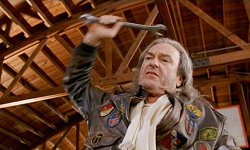
\includegraphics[width=\figwidth]{pics/10/29.png}
	\end{center}
\end{wrapfigure}
We exited the building to see two screaming police officers trying to scramble away from… something.

Imagine a leaking balloon or punctured gas canister, picture the random way it spins and skips around. 
Now imagine that instead of harmless gas it's spraying blue fire. 
Everyone stopped and watch for a second, just trying to figure out what they hell was going on. 
Then Tink screamed at us to watch for the drones.

The drones must have been equally confused by the bouncing plasma gun, because both of them were just hovering over the scene, making them easy targets. 
We shot them down, started piling into the truck, then out again, then in again, then out again. 
Eventually we managed to pull the half-blind Tink out of the driver seat, replace him with the infiltrator, retrieve the now sputtering plasma gun from the between the moaning officers, and drive away before any more police showed up.

As we drove the cogitator adept commed and told us he'd spotted a bulletin for our truck's transponder code, but not its description thank the Emperor. 
So as we drove away at exactly the speed limit and Doc saw to Tink's burns, the techie had to walk Twitch through yanking out our transponder and replacing it with the one Nubby had gotten for us during one of his little walks in the park. 
Once the switch was made we pulled up next to another truck, tossed the transponder into their bed, then drove in the opposite direction at the next intersection. 
A few minutes later the adept confirmed that we'd shaken pursuit and we were clear to return to base.

Sarge breathed a sigh of relief and began filling the base team in on everything that happened and asked what they knew about the planet the Kroot had threatened to send us to. 
While he talked Tink sat on the floor and grumpily poked at his busted plasma gun. 
Fumbles tried to cheer him up and only got a spanner chucked at his head for the trouble.

\begin{wrapfigure}{O}{\figwidth}
	\begin{center}
		
\includegraphics[width=\figwidth]{pics/10/30.png}
	\end{center}
\end{wrapfigure}
The moment we arrived at our warehouse Weebu commed us and requested that we stop by his office, preferably before we did any more damage to his city, planet, or police force. 
Given the timing it was obvious he had someone watching us, so there was no point trying to pretend we were busy, or dead, or not on the planet. 
We got everyone into our backup vehicle, just in case the truck was still hot, and went to get yelled at by a fat old man in a dress.

The ex-Inquisitor wasn't doing the whole peace, serenity, and interracial tolerance tolerance thing today. 
The second we entered he was on his feet and barking like the enraged bulldog of an inquisitor he must have been before all the soft xenos culture went to his head. 
Sarge took the lead and weathered the tirade with his usual stoicism, until Weebu shifted from insulting our idea of subtlety to blaming us for the murder of seven people. 
Sarge firmly denied doing any such thing, playing the serious Interrogator to the hilt, but the effect was spoiled by Twitch and Nubby both adding that "they started it" and "it's not murder if it's xenos anyway, it's like pest control or sumfin." Boy, and we'd thought he was pissed before that.

The tirade went on for a while, other high points included him accusing Tink of attacking two police officers, which Tink firmly denied. 
Phrases like "YOU BLEW UP THEIR CAR AND HOSED THEM WITH PLASMA" were countered with "it was an accident", "I didn't know they kept the fuel there", and "it's their fault for having the flying saucepan shoot my plasma gun." The real clincher was when Weebu listed off the various injuries the officers had suffered and Tink replied that HE'D lost his favorite gun, his eyebrows, AND his best pair of pants. 
That choked up the ex-Inquisitor and started a downward slide from rage to depression.

When he was finally calm, or morose, enough to stop shouting, our adepts stepped in and explained the information we'd gathered.

\begin{wrapfigure}{O}{\figwidth}
	\begin{center}
		
\includegraphics[width=\figwidth]{pics/10/31.png}
	\end{center}
\end{wrapfigure}
The change in Weebu's attitude when we told him where the bounty hunters were taking guardsmen wasn't huge, but it was noticeable. 
He started typing at his cogitator and, in between complaints about how no one under the age of a hundred and fifty understands what patience or subtlety are, asked us to repeat the information. 
He then asked for recorded evidence and testimony from Fumbles that the Kroot hadn't been lying. 
There was a lot of typing and muttering after that and the ex-Inquisitor seemed to forget about us for a while.

Eventually he called a man, asked him to send a report, told him his report was wrong, then told him to get his ass into the office. 
A pale analyst type came in and nearly had a heart attack when he saw the ten of us in there with his boss. 
He nearly had a second heart attack when Weebu introduced us as "a bunch of psychotic man-children from the Inquisition", but rallied quickly when he was asked several socio-political questions about a planet with a name that sounded like a venereal disease.

Honestly, none of us really tried that hard to follow the discussion. 
It seemed pretty important and all that, but we didn't know any of the background and couldn't pronounce half the names involved. 
We all just stood there, hoping the adepts were listening and keeping our mouths shut. 
It sounded like it was a real big deal that the planet in question had recruited bounty hunters and actually wanted deserters to come to their world though.

The discussion ended with all the participants triumphantly agreeing on some point and the analyst being sent to get ten of something. 
Weebu turned to Sarge, assumed the sort of fruity voice he used when he was talking about xenos culture stuff, and thanked us for visiting his planet. 
He appreciated our effort in the investigation, requested that we share any information we uncovered, and hoped we'd visit his humble office next time we were in the system.

\begin{wrapfigure}{O}{\figwidth}
	\begin{center}
		
\includegraphics[width=\figwidth]{pics/10/32.png}
	\end{center}
\end{wrapfigure}
Sarge just stared blankly for a second, the conversation had left him behind about half a klick back. 
He hesitantly agreed that "Yes, the planet was very nice and this office was well decorated," then continued standing at attention. 
Weebu signed, dropped the smile and fruity voice, then told us to "Get the hell off my planet. 
Thanks for the intel, good luck with your mission, don't forget to write, but GET. 
OFF. 
MY. 
PLANET." The analyst came back in at this point and handed over a briefcase then the ranting ex-Interrogator listed all the things he'd be giving us: 
a full copy of their data on the deserters, a dossier on the planet, falsified IDs for all of us, and even tickets on the first commercial transport heading to that planet, all so we could leave as soon as possible. 
In two hours in fact. 
Tick Tock, don't let the door hit you on the ass.

Sarge saluted the man as he stopped for breath, thanked him for his cooperation, and led us out through the back door. 
All in all it went a lot better than we'd expected and the free tickets were an especially nice touch, they'd apparently get us to Syphilis, or Sylphis or however you were supposed to pronounce it, in less than a week. 
Honestly it was the most stylish way any of us had ever been kicked out of a place, we even spotted some government agents redirecting traffic to make sure we got to the shuttleport with time to spare. 
Nubby suggested we try for the same thing on the next planet, if we kept this up we'd be able to pocket half of our operating budget without anyone noticing.

The shuttle ride up was nice and relaxing, with big comfortable seats and no obnoxious questions about what was in our bags. 
We boarded the ship without anyone even asking why Doc looked like he'd been in a bar fight or Tink's face was covered with burn-salve, and were allowed to carry our own bags to a series of cabins reserved for our private use. 
Weebu sure knew how to get someone off a planet without incident.

\begin{wrapfigure}{O}{\figwidth}
	\begin{center}
		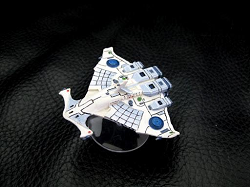
\includegraphics[width=\figwidth]{pics/10/33.png}
	\end{center}
\end{wrapfigure}
It's a commonly known fact, at least if you've suffered through classes on Tau technology, that Tau ships are not as good as Imperial ones. 
This is partially because they are pathetic xenos and everything they produce is inferior to the honest labors of humans, but mostly because they stay the hell out of the warp when they travel and wind up going much slower than an imperial vessel. 
Of course it's a much less well known fact that this makes travelling in one much, much more pleasant. 
Let me tell you, out of the commissar's hearing, that any trooper with the sense he was born with would gladly take a longer than usual void trip over having their soul devoured by daemons.

There were no bad dreams, no bleeding statues, no wordless whispers, and no minor daemonic horrors clawing at the sealed bulkhead to cargobay G19. 
On top of that the ship was clean and well lit, nothing spontaneously exploded or shot lighting at us in the hallways, and if the gravity was a little light, at least it all pointed the same direction. 
It was the best void trip we'd ever been on, at least for the first two days.

We'd been entertaining ourselves in the usual ways and generally avoiding the ship's crew and other passengers. 
Tink tried to fix his plasma gun, Doc tried to fix Tink, Twitch locked himself in one of the bathrooms and refused to come out, and Sarge helped the adepts go through the data we'd been provided. 
Nubby kept making trips to the rest of the ship though, usually taking Fumbles with him, and when a nervous crewmember asked Sarge to please keep them both confined to their rooms, he started asking the infiltrator to visit the rest of the ship. 
We found out why on the fourth day, when, after everyone spent the third day feeling alternately pissy, depressed, and nauseous, Doc took a good look at Fumbles. 


On the list of phrases you never want to hear, "Why is our psyker going through withdrawal?" is pretty high up there.

\begin{wrapfigure}{O}{\figwidth}
	\begin{center}
		
\includegraphics[width=\figwidth]{pics/10/34.png}
	\end{center}
\end{wrapfigure}
Fumbles was a pretty good telepathic psyker, but he had a sort of problem. 
Actually he had a few problems, but the biggest one was that he had couldn't really turn his powers off. 
The psyker tended to broadcast, at a very low level, whatever emotions he was currently feeling to everyone within a twenty meter radius. 
This made him a blast at parties, but could cause some problems at other times, especially if you were stuck for long periods in that radius. 


When we'd first met the poor guy he had a sort of depressive feedback loop going, but he'd been doing much better since he'd partnered up with us, we put it down to positive reinforcement and our squad's fun loving demeanor. 
In retrospect though, the psyker had really started cheering up after he began hanging out with Nubby all the time.

Fumbles apologized for making everyone miserable, but said that Nubby had promised to get him more 'antidepressants' soon. 
Judging by the way everyone's head ached and entire body itched now, Doc was reasonably certain that whatever he'd been taking was a little stronger than an antidepressant. 
When Nubby was pried out of Twitch's bathroom, where he'd fled when Doc first started looking at Fumbles, Sarge hauled him out into the hallway and had words with him. 


The poison of choice turned out to be Gladstones, a moderately strong upper and banned from use by serving guardsmen under section 114b of the Astra Militarum's Laws and Ordinances. 
Possession was five lashes and a month in the brig, distribution was thirty and ten for the first offence, summary execution for the second. 
It wasn't exactly the worst thing he could've been giving the little guy, but they still had some pretty nasty lows, especially considering some of their withdrawal effects could last for months. 


Unfortunately there was not a thriving black market on the Tau merchant vessel. 
Doc did his best with what he had, but saying the rest of that trip was unpleasant doesn't really do it justice.

\begin{wrapfigure}{O}{\figwidth}
	\begin{center}
		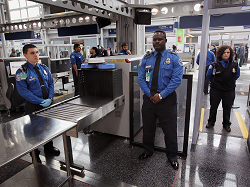
\includegraphics[width=\figwidth]{pics/10/35.png}
	\end{center}
\end{wrapfigure}
After a few more days spent going through withdrawal-by-proxy, we arrived at the planet that we'd agreed to just call pro-Tau world. 
As we got off the shuttle planetside we realized that Weebu's assistance only applied to getting us off of his planet, not onto this one: 
several official inspector types were waiting by the exit and were very interested in what was inside everyone's bags.

There were similar weapons laws on this world as the last one, but this time we didn't have someone in the local government covering for us. 
Sarge desperately tried to think of a way to get around the checkpoint before the rest of the passengers got off and left us standing there alone and obvious. 
Unfortunately, between the time pressure and a pounding headache that was definitely not his fault, the best Sarge could think of was to ask our strung-out psyker to make the guards "forget about us or something." Fumbles gave it a shot, but lived up to his name: 
both us and the checkpoint guards spent the next few minutes trying to remember what we were doing there, why we all felt vaguely embarrassed, and who the miserable looking man sitting on the floor in the middle of us was.

Eventually everyone remembered what was going on and the guards asked us what the holdup was. 
Sarge picked up his bags with a sigh and quietly asked us if we'd rather lose all of our weapons or get in a shooting war with the local government. 
The vote was three to two in favor of surrendering our weapons when the adepts, who hadn't even been asked for an opinion, suggested we let them sort things out. 
We grudgingly let them take the lead, none of us could see any way that talking or cogitator expertise could get us around a planet's weapons laws, but at least it'd let us put off losing our toys or being shot at for a while longer.

Needless to say, we were incredibly surprised when the guards waved us through the checkpoint without an inspection a few minutes later.

\begin{wrapfigure}{O}{\figwidth}
	\begin{center}
		
\includegraphics[width=\figwidth]{pics/10/36.png}
	\end{center}
\end{wrapfigure}
The brainy, talky side of the team was rather smug about getting us through with our gear intact, but they didn't rub our noses in it too hard. 
The old diplomat never did explain how he'd talked the inspectors around, when we asked he just vaguely claimed it was one of the "tools of his trade" and refused to bore us with an explanation. 
We accepted this non-answer and Sarge asked, on behalf of all us guardsmen and himself as the team lead, what we could do to thank them for saving our bacon. 
They suggested that it might be nice to have an actual safehouse, with plumbing and heating and everything, on this planet. 
You know, instead of camping out inside a disused warehouse filled with mines and razorwire again. 
It was a bit much to ask from us, especially Twitch, but never let it be said that guardsmen don't understand the concept of gratitude.

Despite our previous experience, this place was harder to get used to than the last. 
The planet was the most vocal Tau supporter in the cluster, only the odd political situation that forced the whole cluster to hang together kept it from joining the empire outright. 
As it was though, the locals annoyed their neighbors by constantly telling everyone that the Imperium would doom them all and becoming part of the Tau empire was their only hope. 


These guys were obviously trying way too hard to be a Sept, it was probably embarrassing for regular Tau to visit here. 
The signs were in Tau, almost all the buildings were Tau architecture, and you couldn't walk five meters in city we holed up in without seeing posters and billboards about the Greater Good. 
The real kicker though, was that there seemed to be a lot less of the actual xenos themselves here, it was all these weird humans with glazed expressions and stupid hairstyles. 


Surprisingly though it wasn't that hard for us to fit in with the locals. 
You see, the entire place, from the shuttleport, to the streets, to the bloody corner store, was filled with ex-guardsmen.

\begin{wrapfigure}{O}{\figwidth}
	\begin{center}
		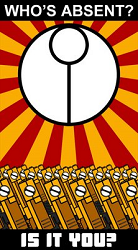
\includegraphics[width=\figwidth]{pics/10/37.png}
	\end{center}
\end{wrapfigure}
Seriously, either Weebu hadn't actually been looking for the deserters over those two weeks, or the guys who got sent here were complete idiots. 
All you had to do was look out the bloody window and there they were, wearing xenos clothing and with the same stupid smiles and haircuts as the rest of the locals, but it was just so incredibly obvious they were guardsmen. 
Hell, even if you didn't know what a guardsman looked like, there were posters every few meters inviting "political refugees" to earn citizenship by signing up with the Guey Vase Washo of Syphilis. 
Or something like that, none of us could pronounce the bloody moonspeak to save our lives. 
We just called it the pro-Tau PDF.

So the local PDF was pretty aggressive about recruitment, especially if you were a guard deserter. 
There were the posters and vid-ads to start with, then there were the pamphlets everywhere, and the worst part was these random people who would walk up to us and ask if we'd enlisted yet. 
Despite all that, it really wasn't as bad as being on an Imperial world during a serious recruitment drive: 
for one thing no one snatched us off the street, drugged us, and threw us into a shuttle for one-way trip to the nearest munitorium world. 
It was still annoying as hell though, it was almost impossible to get the random people to leave you alone if they thought you were a "refugee". 
We wound up putting a lot more effort into disguising ourselves on that planet than anywhere else we'd ever been.

Anyway, we were pretty certain that most of the deserters had wound up on this planet, but it was hard to see why. 
It had been a very long trip to get out here and even if this planet was currently doing a recruitment drive to fight off whatever was raiding the cluster, it was unlikely that they'd been doing it back when all the guardsmen had originally deserted. 


We'd started with the "what" and "when", and now we had the "where", but the "why" and "who" still evaded us.

\begin{wrapfigure}{O}{\figwidth}
	\begin{center}
		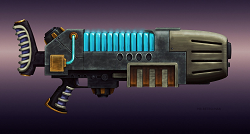
\includegraphics[width=\figwidth]{pics/10/38.png}
	\end{center}
\end{wrapfigure}
Sarge spent a lot of time with the adepts chewing over the data we'd been given by Weebu and the stuff our cogitator adept started pulling off the local comm network. 
It was slow going and we all knew there was a quicker option, but none of us really wanted to try joining the PDF. 
Inserting ourselves into an entire army of well-armed hostiles didn't seem like a good idea.

While Sarge did actual work and Doc tried to deal with the ongoing effects of Fumbles' withdrawal, Twitch did his usual thing and Tink kept trying to fix his plasma gun. 
The techie had met his match though, he just didn't have the tools or knowledge to repair the gaping holes the sniper drone had put in it. 
Watching his expression as he asked Sarge for permission and money to visit a local weapons expert was pretty entertaining: 
you could tell it actually caused him physical pain to admit he needed help. 
The best part was that he even tried to make us promise not to tell the cogboys back on the ship, we lied to make him feel better. 


The only consolation for Tink was that therewasn't a single ordained tech-priest on the planet, he only had to ask for assistance from one of the shorter, fatter variety of local xenos. 


The problem was that while earth caste Tau were wizards with plasma, they also tended to worry about tedious things like weapons laws. 
It took a lot of work to find a disreputable armory, eating up a lot of the cogitator adept's valuable time as well as Nubby's valueless variety, but find one they did and not too far away to boot. 
Sarge gave Tink his cash, and the techile bundled his highly-illegal weapon into a scanproof bag then went out with Nubby and the infiltrator to have some serious tech-heresy committed on his plasma gun.

\begin{wrapfigure}{O}{\figwidth}
	\begin{center}
		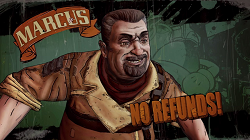
\includegraphics[width=\figwidth]{pics/10/39.png}
	\end{center}
\end{wrapfigure}
The rest of us weren't exactly waiting with bated breath, but when the away team returned everyone came out of their various corners to see how they'd done. 
Tink breathlessly informed us that he had bad news and good news, the bad news was that it'd take at least a week to fix his gun, but the good news was that the repair was being done for free. 
Well not exactly free per-se, but as a sort of bonus thrown in with his other purchase. 
When the rest of us refused to ask leading questions about his "other purchase" the techie triumphantly opened a shielded crate and pulled out a shiny new Tau drone and control system. 


Tink was rather disappointed when none of us gushed enthusiasm over his new toy and got defensive when Doc asked how much it had cost. 
Sarge took a long look at the complex device, thought about how tight fingered the Tau were when it came to their fancy technology, and growled at Tink to answer the damned question. 
The techie hesitantly admitted that he hadn't really looked that hard at the price tag, "I mean it had so many features, why get hung up on something small like price," but assured us that it had fit perfectly into the budget Sarge had given him. 
Doc winced as he recalled how Sarge had just handed over their briefcase full of xenos money and told Tink to take what he needed, then led the retreat.

As reamings went, the one Tink got for spending three quarters of our mission's budget was pretty nasty. 
Nubby and the infiltrator weren't spared it either, Sarge said that between the three of them they should have had at least one functioning brain. 
Eventually he wound down and plaintively asked if there was any chance of getting a refund, voluntarily or otherwise, but all three idiots said the black-market armory had a fairly strict no returns policy and some really heavy security. 
In the end Sarge just put them in charge of making the cash back.

Looking back, that decision was where things started to really go off the rails.

\begin{wrapfigure}{O}{\figwidth}
	\begin{center}
		
\includegraphics[width=\figwidth]{pics/10/40.png}
	\end{center}
\end{wrapfigure}
Nubby was fairly good at making money, but the competent local police force made it hard. 
He and the infiltrator did what they could, but weren't making much headway and Tink was flat out useless. 
He kept running off to check on his plasma gun and talk to the earth caste weaponsmith, who he'd decided was female. 
The rest of us couldn't tell one xenos gender from the other, assuming they only had two that is, and found this even more revolting than his usual behavior around female tech-priests. 
It kept him out of trouble though and she/he/it gave Tink several lessons on using his fancy new scouting drone.

So anyway, Nubby and the infiltrator were having trouble refilling our budget and in the end they asked for help from the rest of us. 
Well, to be more specific they asked for help from Doc, who was currently acting as Fumbles' Sargeally-Appointed-Guardian. 
Nubby claimed he and the psyker had a good scam set up on the last planet, it involved passwords, numbers, and the xenos banking system and didn't require any violence at all. 
All he needed to get it running again for Doc to release Fumbles from his medical clutches, despite the fact that the little guy was still suffering fairly badly from withdrawal.

Doc considered the situation carefully, weighing his patient's current condition against the team's need for funds and how nice it would be to get out of the psyker's aura for a while. 
In the end he extracted a promise from Nubby not to give Fumbles any more Gladstones, then sent the little guy off with the rest of them when they left the safe house the next morning. 
If he'd listened carefully he might have heard Nubby telling Fumbles that Doc wouldn't mind if they got a little pick-me-up as long as it wasn't Gladstones, and they could even make a little profit while they were at it.

Yeah, so that's how four members of our crack Inquisitorial investigation team got arrested for trafficking prohibited substances and sent to Ethical Re-education Camp.

\begin{wrapfigure}{O}{\figwidth}
	\begin{center}
		
\includegraphics[width=\figwidth]{pics/10/41.png}
	\end{center}
\end{wrapfigure}
It took a while for the rest of us to figure out what had happened. 
The first hint was when the Tau weaponsmith called us, Emperor knows why the idiot gave that xenos our comm codes, and asked why Tink hadn't shown up to pick up his plasma gun. 
Sarge thought she actually sounded concerned and made a note to have a chat with the techie about the birds, bees, and Inquisition's stance on fraternization with xenos, then promised to comm Tink and see what was keeping him.

Tink's comm was active, but he wasn't the one who answered it. 
One of the locals who was too stupid to understand Gothic babbled at Sarge until he handed the comm over to the xeno-expert adept. 
The adept exploded in a flood of Tau, ignoring Sarge's questioning looks and waving the other adepts over to listen in.

There was a lot of talking, a bit of shouting, and a general air of extreme panic; 
Sarge knew what it looked like when people were doing their job and provided some very real assistance by keeping Doc and Twitch from asking what all the noise was about. 
When the call finally ended, in our favor from the sound of it, and the adepts stopped hyperventilating, they informed us that Tink's combead was currently being held by the pro-Tau PDF. 
It would be returned to him with the rest of his gear after he finished basic re-education and became a full member of the PDF. 
Sarge facepalmed.

\begin{wrapfigure}{O}{\figwidth}
	\begin{center}
		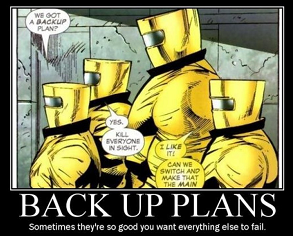
\includegraphics[width=\figwidth]{pics/10/42.png}
	\end{center}
\end{wrapfigure}
A little cogitator work established that the rest of their comms were in the same location and turned up the arrest report. 
Doc swore loudly and venomously when he noticed what they'd been arrested for and Twitch suggested that Fumbles' addiction was actually part of a complex xenos conspiracy to split us up and pick us off like this. 
Sarge told both the troopers to stuff it and called an emergency planning session. 


The available options were limited, either we busted them out before the xenos messed with their brains or rolled with this like it was our plan to infiltrate the PDF all along. 
If we went with the former we needed to figure out a way to pull it off without blowing our cover to hell and bringing an entire army down on our heads. 
If we went with the latter we needed to decide whether to all go in together or figure out a way to get in and make contact after the idiots went through their brainwashing. 
The adepts suggested going in together, probably because it'd get us out of their hair sooner, and Doc was in favor of figuring out a way to infiltrate without getting brainwashed ourselves. 
Twitch was the only one who wanted to mount a rescue operation, but his whole plan was to just blow up as many PDF buildings as possible, pull our guys out of the rubble, then declare the whole mission a success. 
Sarge made that Plan B.

In the end Sarge sided with Doc and we set up an observation post near the PDF's main base in the city. 
The basic theory was that we'd keep an eye open for ways to infiltrate and otherwise just wait for the latest batch of recruits to finish their brainwashing and get dumped there. 
Once we spotted some new faces in the base we could look harder for our boys and see if they were in any condition to help us get in. 


\begin{wrapfigure}{O}{\figwidth}
	\begin{center}
		
\includegraphics[width=\figwidth]{pics/10/43.png}
	\end{center}
\end{wrapfigure}
In this case Observation Post was mil-speak for a caff-shop with a good view of the base's entrance. 
We spent two weeks taking turns sipping bad recaff and pretending to work on data slates while we watched incoming traffic. 
Luckily we didn't have to pay too much attention, the cogitator adept had taken ownership of Tink's drone and sent it up to the top of a neighboring building. 


Honestly the drone saved us a lot of effort, it did most of the tedious watching and told us when interesting stuff was about to happen, all we had to do was be there to double check things. 
We didn't even have to worry about it being spotted, the thing had this wonderful little stealth field built in, you couldn't see it at all if it didn't move. 
We considered forgiving Tink for paying so much for it, then remembered why we were in our current situation and how unbearably awkward it had been collecting his gun and explaining his disappearance to the Tau weaponsmith.

After two weeks of watching and some careful hacking from the cogitator adept we had a few ideas for getting into the base. 
The plans ranged from simple, to complex, and their success chances varied based on whether our teammates on the inside would be able, or willing, to help us get in, so we prepped for them all and waited to see how things would turn out. 
When a load of fresh recruits finally arrived and we spotted the sawed off form of Nubby jumping out of a truck we got ready to move, and tried our best to make contact.

Unfortunately it was damned hard to get a message into the base and it seemed like fresh recruits weren't allowed to leave. 
We were on the edge of trying the horribly bad idea of calling their sure-to-be-monitored combeads and talking in code or something, when a senior looking PDF trooper walked right up to us in the caf-shop. 


Twitch nearly shot our infiltrator, sometimes it was easy to forget that we had a teammate who was supposed to be a master of disguise.

\begin{wrapfigure}{O}{\figwidth}
	\begin{center}
		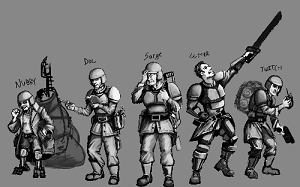
\includegraphics[width=\figwidth]{pics/10/44.png}
	\end{center}
\end{wrapfigure}
According to our infiltrator the locals weren't anything special when it came to brainwashing. 
All four of them had come through the process intact, mostly, and even had had their gear returned. 
They had duties to perform in the base and were under a little observation for senior PDF members, but should be able to get us in without much trouble as long as we acted like guardsmen. 
He didn't think this would be hard for us.

The next day the infiltrator returned to us with some of the tau-ish flak armor and tan fatigues that the locals wore, as well as some military IDs that only needed a little doctoring. 
He didn't even need to provide authentic PDF weapons, apparently until you were issued a fancy Tau gun you were allowed to keep whatever you were originally trained with or switch for a nice local-made lasgun. 
The only thing that couldn't be carried right in the front door was our few heavy weapons Twitch's stuff, no matter how open minded you were it was hard to ignore twenty five kilos of high explosives. 
Luckily, the infiltrator claimed he could get at least one scan-shielded bag in if we needed it.

We sent Sarge's nade launcher, Tink's stupid plasma gun, and as many explosives as could still be fit in the bag ahead, then finalized or plans with the adepts. 
They'd be staying in the safehouse and monitoring us of course, but the problem was that the PDF had some sort of fancy Tau jamming field over their base. 
It blocked any unauthorized communications, so while the adepts could watch and plan, they couldn't talk to us or provide real assistance if shit went south. 
Our theory was that they'd just sit, collect data, and keep working on figuring out why the deserters were here while we were inside. 
If they found something important they'd and send Tink's drone to find us, if we saw one of our targets we'd send the infiltrator out to find them.

Our plan, as it was, finalized we suited up and just walked right in the front gate of the PDF base.

\begin{wrapfigure}{O}{\figwidth}
	\begin{center}
		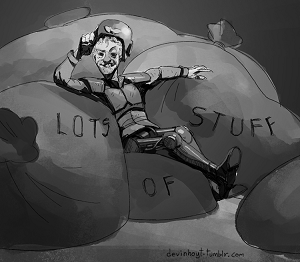
\includegraphics[width=\figwidth]{pics/10/44b.png}
	\end{center}
\end{wrapfigure}
So no shit there we were, undercover in the middle of a bunch of xenos-loving traitors, and the main thing we noticed was that the place was almost exactly the same as a normal guard camp. 
Sure it was a little cleaner and there was a bunch of Tau tech lying around, but if you ignored the fact that all the officers were short, blue, and had drones hovering around them, it all felt completely normal. 
Everyone was doing the usual chores or drills, the gear was practically identical, and the food wasn't even better. 
It was a wonder that these people had even bothered to desert, they were still in the bloody army weren't they?

The first thing we did after entering was collect our teammates and verify that they were in as good condition as the infiltrator had said. 
Tink and Nubby were absolutely fine, in fact they'd fallen right back into their usual roles when in base. 
Which is to say Tink was in the armory disassembling a Tau gun that he shouldn't have had access to and Nubby was sitting on an impressive cache of stolen or bartered goods in a disused supply shed. 
Nubby claimed that if he could find a buyer with actual cash he was halfway to refilling our budget.

Neither of them were trying particularly hard to act brainwashed, whoever was the brains of this operation wasn't working counter-intelligence. 
After they established that you were a guard deserter they stopped looking for anything else and welcomed you in with open arms, after that it was just a matter of parroting all the Greater Good stuff. 
You didn't even need to parrot it well or speak the language properly, if you screwed it up they just assumed you were an idiot.

Speaking of idiots, neither of the guardsmen had bothered keeping track of Fumbles, claiming that he wasn't in any shape to cause trouble. 
This didn't sound very encouraging, but Sarge refrained from slugging them and we all went to find our psyker before he did something warpy.

\begin{wrapfigure}{O}{\figwidth}
	\begin{center}
		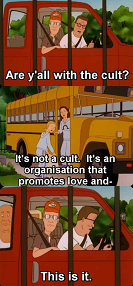
\includegraphics[width=\figwidth]{pics/10/45.png}
	\end{center}
\end{wrapfigure}
We found Fumbles sitting in a circle of PDF troopers and singing, if you'll believe it. 
He was wearing the same dopey expression as the rest of them and a sort of idiotic happiness radiated off of him. 
He happily introduced us to his new friends and asked if we wanted to lead the next song. 
Sarge eyed the large group of smiling armed men, then politely declined and asked if he could borrow Fumbles for a while. 
No one put up a fuss as we dragged the psyker away and we all kept smiling and nodding until we got around a corner, where Sarge started quietly dressing down Tink and Nubby.

Doc took a good look at Fumbles and declared him to be low on sleep, low on protein, and high on something that was probably a Tau drug tailored to help with withdrawal symptoms. 
He claimed that a little talking, some basic care, and a slow reduction of the detox drug, the bottle of which he took immediate possession of, would sort the psyker out in a few days. 
For now though, it was probably best if he stayed in Nubby's storeroom when he wouldn't be missed.

Our team finally collected we sat around our dopey psyker and tried to plan our next step. 
Our end goals were still the same: 
find out why so much trouble had been put into getting the deserters out here to join the PDF, find out who the Tau that had led them was, kill him and every senior defecting officer as well as the rogue trader if he was still around. 
In the short term all we could think to do was fit into the routine in the base and use every bit of free time we got to ask discrete questions. 
We probably wouldn't get anything from most of the troopers or the Tau officers, but if we got access to the command building at the far end of the base we might find someone who knew something.

\begin{wrapfigure}{O}{\figwidth}
	\begin{center}
		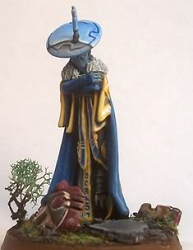
\includegraphics[width=\figwidth]{pics/10/46.png}
	\end{center}
\end{wrapfigure}
Over the next week we mostly we learned how easy basic training was after you'd already done it once and how awesome everyone thought the Greater Good was, but there were a few useful things mixed in. 
We managed to spot the Traitor General we'd seen on our last mission leaving the command building one night, learned that there were occasional meetings with a big-league Tau politician in said command building, and found out that the Tau Fire Caste who led this PDF army was a loan from the Empire and a personal friend of the politician. 
In fact they were so friendly that a team of Fire Warriors under his command was permanently assigned to protect the politician. 
We suspected that the diplomat was the cloaked xenos who'd led the desertion plot, but weren't quite certain.

We also had a decent lead on the rogue trader. 
Mostly the camp was all smiles and songs, but occasionally the fresh recruits that were dropped off didn't fit in. 
They weren't put through a second brainwashing or quietly executed, like they would've been back in the guard, instead they were put on a shuttle that left once a week and took them to a "mercenary outfit" outside the cluster. 
It sounded fishy as all hell, but some careful scanning by Fumbles proved the the officers really believed it. 
So if there really was a mercenary company we figured it was probably owned by the rogue trader that'd been part of the desertion plot. 
It's a well known fact that you can't get much more mercenary than a rogue trader.

\begin{wrapfigure}{O}{\figwidth}
	\begin{center}
		
\includegraphics[width=\figwidth]{pics/10/47.png}
	\end{center}
\end{wrapfigure}
So if the mercenary was really the rogue trader, there were only three things that we still needed to figure out. 
First, was the location of the remaining traitorous guard officer, he was just a major, but he still needed to die. 
Second, we needed proof that the Tau diplomat was the cloaked xenos so we could be sure we'd gotten the whole set. 
Finally, we still had no idea what the hell this was all about. 


As far as everyone we talked to knew the army's only purpose was to protect the planet from whoever was raiding the cluster. 
This sounded fairly reasonable, especially considering that even more raids had been reported over the months of our mission and gotten all the civies worked up, but we knew it was at least partially bullshit. 
The desertions had started happening way before the raids, so there was obviously something else going on, even if we were too stupid to figure out what it was. 
Luckily we'd brought some smarter people along just for this sort of thing.

We sent out the infiltrator with all of our data and the adepts did a little digging. 
Mostly they looked into the Tau politician, since he was both the public face of the whole operation and the suspected mastermind behind the desertions. 
According to them he was an off-worlder who'd come from the Tau empire and was one of the guys yelling the loudest for the cluster to join or ally with them. 
As far as us guardsmen could tell this made him an asshole, but didn't prove he was our guy or explain what was going on, the diplomatic adept insisted it all made sense though. 


In the end he had to dumb it down a little before we really followed the situation, and by "dumb it down" I mean he sent us a vid of him acting out with freakin sock puppets. 
There was a blue sock that was supposed to be the Tau politician and a tan one that acting as the rest of the cluster's political leaders.

He seemed to be enjoying the fact that we couldn't easily leave the PDF base and throttle him.

\begin{wrapfigure}{O}{\figwidth}
	\begin{center}
		
\includegraphics[width=\figwidth]{pics/10/48.png}
	\end{center}
\end{wrapfigure}
>Hi I am the Tau politician guy who might also be the secret mastermind behind the deserters

Hi politician guy, I'm all the other politicians in the cluster. 
We are scared because raiders have been attacking our planets.

\greentext{>I think we should join all voluntarily join the Tau empire for their protection}


We don't know, we like being independent and worry that the either empire will change our way of life and start a war

\greentext{>Well we have to do something to protect ourselves, there's no point avoiding a war if we all die to raiders.}


Hmmm, if our armies aren't holding of the raiders and we have to join an empire, the Imperium is bigger and scarier.

\greentext{>I don't think they would protect you, the Imperium doesn't care about anyone but humans and I hear the raiders are all humans, maybe they even work for the Imperium!}


That's worrying, but we still don't want to join the Tau empire

\greentext{>Well I can't force you to join the Tau empire, but what if you accepted their assistance arming and training your armies? You'd be able to protect yourselves and there wouldn't be any big Tau Empire military bases to provoke the Imperium into war}


That doesn't sound much better than our own armies, and it would give the Tau empire a lot of influence over us

\greentext{>No it IS much, much better. With superior Tau weaponry and training your armies can easily handle the raiders. See, look at my army here.}


That army looks impressive, but we still aren't sure it would do anything to stop the raiders.

\greentext{>Watch, if the raiders show up near us, we'll kick them back off the planet and chase them out of the system.}


Hmm if that works we might listen to you about forming a partial alliance with the Tau Empire. 
Goodbye now.

\greentext{>"HAHAHA, My master plan will make them all into slaves of the evil Tau empire.}


\begin{wrapfigure}{O}{\figwidth}
	\begin{center}
		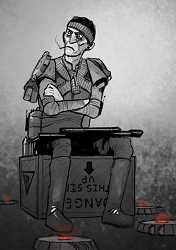
\includegraphics[width=\figwidth]{pics/10/49.png}
	\end{center}
\end{wrapfigure}
So getting our critical mission data via sock puppets was demeaning as hell, but it got the point across better than the giant documents they'd originally sent. 
When the show was finished we sat down together in Nubby's store room and chewed the situation over, trying to figure out what all the political info meant for us and what our next step should be.

Sarge wound up deciding to go with Twitch's current interpretation of events, which for once seemed fairly reasonable. 
His theory was that if the politician was the one who'd orchestrated the desertion and dragged them all the way out here, he was probably behind the raids too. 
What's the point of having an army if it doesn't have anyone to fight? 
This theory neatly placed all the blame on one person, so if push came to shove we could just kill him and call it a day.

Of course, this all sort of hinged on us the politician being the cloaked xenos, and Oak was probably not going to accept "we were pretty sure" as proof of mission completion. 
Furthermore, when we shared our general plan with the adepts they insisted that we prove that the politician was behind the raiders instead of just killing him. 
They said that, given how many people had died in the raids, it would be a huge blow against the Tau empire if we could prove they, or at least their supporters, were behind everything. 
This sounded like the sort of thing that the Inquisition was supposed to do, so Sarge reluctantly agreed and we started planning ways to spy on the meetings in the command building instead of just blowing it up. 
Twitch was disappointed.

\begin{wrapfigure}{O}{\figwidth}
	\begin{center}
		\includegraphics[width=\figwidth]{pics/10/50.png}
	\end{center}
\end{wrapfigure}
Sneaking into the command building turned out to be much easier than it'd originally looked like. 
Sure, there were Tau guards on the doors and most of the staffers were slit-heads too, but the place was cleaned and maintained by the recruits. 
At first we'd thought that it would be necessary to get ourselves on the duty roster to get inside and started figuring out how to arrange than, but then we found out the guards weren't checking IDs and apparently couldn't really tell one human from another. 
Hell, it seemed like their only real purpose was to keep anyone from entering the building armed and they did that using a simple door scanner. 
A quick check even revealed that it was the same type of scanner we'd already fooled multiple times with scan-shielded bags and clothing.

So yea, it was pretty apparent that whoever was running security on this operation wasn't the brains of the outfit, or they were terminally trusting, or both. 
Anyway, we didn't look a gift-horse in the mouth, and quickly put together a straightforward plan for getting what we needed and getting out. 


We would figure out when the politician was coming for a meeting, bug the conference room, record him saying some really incriminating stuff, go in after the meeting and retrieve the device, then hand the recording over to the adepts and see if it was what they wanted. 
If that went smoothly then we'd be clear to wait for his next visit then grab him or the Traitor General when they went to the bathroom and have Fumbles rip the locations of the rogue trader and last traitor officer from their minds. 
After that we could just blow the entire building up and escape in the confusion. 


It was a nice, simple plan, and we'd have everything in place for our backup strategy of just blowing the building up. 
The only way it could go wrong was if we'd missed something major or one of us completely screwed up. 
Unfortunately we did both.

\begin{wrapfigure}{O}{\figwidth}
	\begin{center}
		\includegraphics[width=\figwidth]{pics/10/51.png}
	\end{center}
\end{wrapfigure}
The thing we missed was the fact that the politician's bodyguards took their job far more seriously than the other guards. 
When they entered the conference room they didn't just do a quick visual sweep, they took out scanning tools and checked the place for power sources and data connections. 
Tink's little home-made bug showed right up and the scanning guard went over to check it out. 


Meanwhile our entire team, sans adepts of course, was in the supply room on the other side of the wall listening in. 
Tink swore, told us we were busted and recommended we bail before they did a search of the building. 
Nubby and Twitch were already halfway to the door when Sarge vetoed this and told Fumbles to take a shot at fixing things. 
The psyker lined up his target using the visual feed and his own ability to sense emotion then psychically commanded the bodyguard to forget what he was doing and go back to his post. 


He'd performed that particular mental trick twice already during our infiltration, but this time, right at the critical moment, Fumbles fumbled. 
Our entire room and conference room's adjacent wall were instantly covered by a sheet of frost. 
That didn't phase the bodyguard Fumbles had been aiming for, but there a few other people in the room. 
While the other bodyguard drew his weapon and covered the wall the Fire Caste who led the PDF warned everyone there was a psyker nearby and told them to get out. 
Then, I shit you not, the Traitor General yelled "It's Bane Johns, I told you he'd never stop chasing us", grabbed the politician, and sprinted out the door. 
It would've been hilarious if we weren't all so screwed.

\begin{wrapfigure}{O}{\figwidth}
	\begin{center}
		\includegraphics[width=\figwidth]{pics/10/52.png}
	\end{center}
\end{wrapfigure}
None of us even tried to stand and fight, we knew a FUBAR mission when we saw one. 
If they had any brains their next steps would be to seal the base and start an exhaustive search for us, and if they remembered Bane Johns they probably remembered what we looked like, so trying to blend in like we had been wouldn't work. 
We either needed to make it out of the base before they locked down the exits, or find a damned good hiding place in the base. 
First thing first though, we needed to get out of the building before we wound up trapped in it.

Nubby and Twitch led us in an all-out sprint for the least guarded building exit, we were probably halfway to the door before the bodyguards or PDF commander even thought to enact some sort of lockdown. 
Of course seven men running through the hallways at a dead sprint attracted some unwanted attention, and we really couldn't afford to have anyone speeding up the search right now. 
The infiltrator plugged a dumb recruit who got in our way with his silenced pistol, Sarge's clothesline broke the neck of a second, and wwo Tau staffers died with surprised expressions on their faces and combat knives buried up to the hilts in their foreheads. 
Twitch and Nubby didn't even stop to pull their knives back out, there wasn't time. 


We hit the door about twenty seconds before the alarm sounded. 
The single Tau guard watching it started to draw his weapon, then Fumbles did something irreversible to him and he forgot we were there and most of his childhood to boot. 
We all felt a pang of guilt from the psyker, quick and dirty psyking isn't pretty stuff, but at least that was the last casualty. 


We could see the base's gates closing ahead of us, so at Sarge's signal we slowed down, fanned out, and tried to look nonchalant as we walked towards Nubby's storeroom. 


\begin{wrapfigure}{O}{\figwidth}
	\begin{center}
		\includegraphics[width=\figwidth]{pics/10/53.png}
	\end{center}
\end{wrapfigure}
There wasn't time for a long debate about what to do next, the options were: 
find a way out, hide, or fight to the death. 
Twitch suggested that enough explosions would distract the gate guards, but Tink shot that down when he pointed out that the perimeter drones would never leave their post. 
Nubby volunteered a few hiding places, but even he wasn't confident they'd hold up to a serious search. 
Tink and the infiltrator started putting together a half baked plan to impersonate an officer and steal an APC from the motor pool, then were interrupted when Doc sprang to his feet and told everyone to shut up.

Doc told the rest of us that wasn't much time to explain, the only way his idea would work was if we moved fast. 
We grabbed what gear we could easily carry and followed the medic as he led us towards the middle of the base. 
As we half-ran Doc quietly explained that there was one exit that was never well sealed, because it was supposed to be "open to everyone, free of judgement or reproof." The weekly shuttle that took the few troopers that refused to embrace to Greater Good to their new life as mercenaries had landed that morning and it was still on the pad.

There weren't expensive drones watching the shuttle, or even Tau guards, just a pair of recruits who were supposed to ask anyone if they were really sure they wanted to leave. 
Doc figured that if we got on the shuttle before the serious search started and the guards vouched that no one had come past them, then it'd be allowed to leave on it's normally scheduled run. 
All we needed for this to work was a bit of luck, a little sloppiness from our pursuers, and for Fumbles to pull off two more pieces of psyking. 
At the back of our group the Fumbles realized this entire plan rested on him and made a small choking sound.

\begin{wrapfigure}{O}{\figwidth}
	\begin{center}
		\includegraphics[width=\figwidth]{pics/10/54.png}
	\end{center}
\end{wrapfigure}
We got Fumbles calmed down and took up position a little way away from the shuttle ramp. 
Each of us told the nervous psyker we believed in him, then Doc gave the signal and everyone held their breath. 
One guard's expression immediately went vague, but as Fumbles turned towards the second a sort of dark foreboding, it felt as if everything was about to come crashing down around us.

It didn't though, the second guard's expression went vague too, then we shook off the uneasy feeling and casually walked up the ramp. 
Fumbles practically collapsed in relief when we turned the first corner. 
Everyone took turns quietly congratulating the little guy as Nubby led us to a convenient spot for hiding unofficial cargo on this model of shuttle. 


Our wait in that dark little compartment was long and nerve wracking, but it wasn't interrupted. 
A few hours after we boarded the shuttle started making it's pre-takeoff noises and we all started breathing a little easier. 
Nubby pointed out that it seemed Fate was with us today and got told to shut up by everyone else.

Since we seemed to be out of the woods Sarge started thinking about the mission again. 
Despite the way we'd been forced to scrub the current op, the mission as a whole wasn't beyond salvage and, all in all, we were getting some good intel from this screwup. 
In our minds the Traitor General yelling about Bane chasing "us" confirmed that the Tau politician was the cloaked xenos. 
Furthermore, we were on our way to confirm that the mercenary was company was actually the rogue trader and would probably behind the raids as well. 
As for the rest of our objectives, hopefully all the time it'd take us to get back from wherever this shuttle was headed would let the situation groundside cool down enough for us to make another attempt.

Of course there was the whole "traveling between planets without our own spaceship or funds" thing, but that was just details. 
We could work it out on the fly.

\begin{wrapfigure}{O}{\figwidth}
	\begin{center}
		\includegraphics[width=\figwidth]{pics/10/55.png}
	\end{center}
\end{wrapfigure}
As we lifted off Doc asked a question that hadn't occurred to anyone else: 
what the hell were the adepts going to think when we just disappeared? 


He worried that the adepts might do something stupid to try and rescue us if they thought we'd been captured, they really needed to be told what had happened. 
Sarge winced at the thought and pointed out we couldn't comm them, the PDF jammed everything but their own, well monitored, frequencies and our short range comms wouldn't work from space. 
While everyone speculated on how much it was going to suck for the adepts and whether it was worth it to try and sneak onto the shuttle's bridge and us their vox, Tink ripped out his combead and jacked it into the pocket dataslate he carried. 
A few seconds later he scared the shit out of everyone by yelling and jumping.

Once Twitch and Fumbles had been calmed down Sarge grilled Tink on what all the excitement was about. 
The techie triumphantly told us he'd managed to get a plaintext message out on the public channel between the time we left the PDF's jamming radius and got out of the local comm net's range. 
Doc congratulated him asked what he'd said in the message, only to get a lot of vague answers. 
Nubby yanked the dataslate out of Tink's hands and read it off to us.

\greentext{>Mission went sort o fb ad, were fine, going 2 space 2 hide adn investgate b back in asap to try agian. tell earthcast grl im ok, keep doin stuff -TINK}


It was probably better than nothing.

\begin{wrapfigure}{O}{\figwidth}
	\begin{center}
		\includegraphics[width=\figwidth]{pics/10/56.png}
	\end{center}
\end{wrapfigure}
The shuttle docked after a few hours of travel and we snuck out of our hidey hole. 
A quick peek around revealed that everyone, even the pilot, had left the ship and no one was guarding the exit. 
We hurried through the hatch and found ourselves standing in a fairly dingy shuttle bay that looked like it was part of an Imperial style ship: 
It had the prayer seals and skulls and everything. 
Tink made a quick check to see if we could steal the shuttle, but the bay doors were locked. 
Sarge decided it was probably time to do a little exploring and nearly headbutted a crewman as he peeked out into the passageway.

The crewman didn't shout an alarm or act more surprised than you usually do when you nearly get a concussion, that probably saved his life. 
Instead he asked if we were the last ones from the shuttle and pointed us towards the bay where all the other "dirtsuckers" were staying. 
Before we followed his directions Nubby traded the man some smokes for a rundown on the ship and more info about our fellow passengers. 
Apparently it was just a tramp freighter that plied the well mapped warp lanes in the cluster and there were about forty other ex-PDF on board. 
He really did say "about", no one on the ship really paid much attention to their passengers as long as they stayed in their area. 
That suited us perfectly and we happily went to join our fellows.

It was remarkably easy for us to blend in with the ex-PDF, no one asked us questions or even paid us much attention. 
We commandeered a pair of the partially furnished shipping containers that were acting as passenger quarters and made ourselves comfortable. 
A few hours later we felt the ship's engines kick on and that night we jumped into the warp, all without anyone saying more than ten words to any of us. 
We'd missed this sort of apathy in the PDF base, it was nice when no one gave a shit about what you did.

\begin{wrapfigure}{O}{\figwidth}
	\begin{center}
		\includegraphics[width=\figwidth]{pics/10/57.png}
	\end{center}
\end{wrapfigure}
Traveling to the "mercenary outfit" took four days. 
We spent them maintaining our gear and forming vague plans for the next stage of the mission. 
Our neighbors mostly spent them drinking to drown out the whispers of warp travel, casually bitching about how the Tau were a bunch of sissies, and speculating on how much money and sex they'd get as a mercenary. 
It was a very homey environment.

When we finally exited the warp a crewman came down and directed everyone towards a shuttle bay. 
The few ex-PDF who appeared to be having second thoughts or were too drunk to walk there themselves were dragged along by cargo servitors. 
One short shuttle ride later we were in a bigger and much more grandiose bay being welcomed to a new life filled with money, violence, drugs, xenos killing, sex, and more money. 
The mercenary really did make a good recruitment pitch, especially the part where he parrotted the PDF's line about being free to leave at any time while gesturing at an airlock. 


By the end of the speech everyone seemed to understand the situation and snappily fell into line behind a few grizzled veteran types. 
Most of the rest of the day was spent in orientations of one sort or another and the usual army recruitment stuff. 
Uniforms and bunks were issued, schedules were handed out, and one or two random men were mercilessly screamed at for minor and possibly imaginary infractions. 
Sarge watched all this with an approval that was only slightly marred by the fact that the yeller was a vile traitor to the Imperium instead of an honest guardsman.

To no one's surprise, the uniforms worn by the mercenaries were perfect matches for the one's we'd seen on the guards in a certain villa. 
Between that and the night's festivities we had all the proof we personally needed. 
Seriously, it was announced as a "Celebratory post-raid feast. 
Don't forget to bring your best loot to show off."  Some rogue traders really don't go in for subtlety...

\begin{wrapfigure}{O}{\figwidth}
	\begin{center}
		\includegraphics[width=\figwidth]{pics/10/58.png}
	\end{center}
\end{wrapfigure}
There was a speech before the feast, it was given by the rogue trader and involved a lot of words like pillage and plunder. 
While everyone else was busy listening Sarge asked the infiltrator, who was the only one of us the trader hadn't seen before, to try getting close to the senior officers and finding out where we were headed next. 
The man practically vanished as soon as Sarge gave the order; 
later we saw a familiar looking server at the trader's high table, but we really weren't sure it was him.

So while the infiltrator did the actual work we enjoyed the party, there wasn't really much else to do. 
We ate, swapped some old war stories with the mercs, and successfully hid the fact that we weren't drinking. 
Much.
Sarge kept an eye on all of us, making sure we stayed under control, and covering for Doc when the mercenaries' tales of horrible violence on defenceless xenos made him sick. 


The party finally petered out at about four in the morning and we all regrouped with the infiltrator in a handy nook Nubby had discovered. 
He had three important pieces of intel for us. 
Firstly, our next destination was the pro-Tau world we just left and the trader with his fast, navigator controlled ship, was aiming to get there in two days. 
Secondly, the official commander of the mercenaries matched our description of the final traitorous guard officer to a T. 
Finally, the raid would not start immediately upon arrival: 
the ship's Seneschal and the traitor officer would be going down "make sure everything is in order with our employer." Sarge thought that sounded like the ideal time to get off the ship.

Slowly, in the wee hours of the morning, a plan came together. 
Mostly it was simple and straightforward, but Doc suggestion for dealing with the rogue trader was downright evil. 
None of us could look him in the eye after he made it, the boy clearly had been corrupted by his time with the rest of us.

\begin{wrapfigure}{O}{\figwidth}
	\begin{center}
		\includegraphics[width=\figwidth]{pics/10/59.png}
	\end{center}
\end{wrapfigure}
We had just over two days to get everything together for our plan, but we managed most of it that first night. 
It wasn't until about noon that someone started imposing order on the mercenaries, so we had free run of their section of the ship, allowing us to get almost all the supplies we needed. 
Over the next two days we used a combination of bribery, intimidation, and good old fashioned lying to avoid most of the chores the other mercenaries were doing and wander around the ship undetected. 


Sarge split us into two teams for most of the work. 
He, Nubby, and Doc concentrated on getting everything set up for our shuttle ride with the Seneschal while Tink and Twitch were escorted on their mission by Fumbles and Infiltrator. 


Our time on the Occurrence Border really paid off for us during those days: 
we found in much easier to navigate this ship than any of the other mercenaries did. 
The maintenance passages and little locked doors that the crew used to get around quickly were an open book to us, we popped up in places that none of the crew even suspected a dirtsucker could get to. 
We made a complete mockery of their security and accomplished all of our objectives without ever being noticed, much less stopped.

Our preparations were finished well ahead of schedule and at Sarge's urging we all got a full night's sleep, or as close as you can get to on a ship travelling in the warp, before the big day.

\begin{wrapfigure}{O}{\figwidth}
	\begin{center}
		\includegraphics[width=\figwidth]{pics/10/60.png}
	\end{center}
\end{wrapfigure}
The Seneschal, being a Seneschal and therefore the very definition of a crafty bugger, probably knew his crew and the mercenaries engaged in a little smuggling. 
He probably wrote it off as a perk of their job and turned a blind eye, so long as they didn't cause him any trouble that is. 
What he didn't know though, was that this time the little smuggling bay on his shuttle wasn't being used to transport a few crates of proscribes substances and weapons. 
This time it was transporting seven crates, each of which held a very uncomfortable inquisitorial agent.

The smugglers didn't know what was in the crates either, but they'd been given clear instructions not to open them and stood to make a lot of money on this deal. 
Upon landing they were to take these crates to a certain supply shed, use a code they'd been given to get in, and exchange them for several of the crates full of PDF hardware that filled the room. 
The boys were professionals and did their job smoothly and speedily. 
Once they were clear Fumbles gave us a signal and we all emerged in Nubby's storeroom, which was a little emptier than it should have been, but it wasn't like we'd even owned that stuff anyway.

The first, well actually second, phase of our plan completed, we started prepping for the hard part. 
The first hiccup came when we sent the infiltrator to contact the adepts and retrieve Tink's drone. 
He got through fine, but the news he delivered wasn't exactly good. 
Well most of the stuff from the adepts wasn't bad, they'd gotten Tink's message and kept everything under control, but there was a message from Weebu as well. 
Apparently several ambassadors from other planets in the cluster were here to observe the PDF and the ex-Inquisitor had tagged along with his delegation.

\begin{wrapfigure}{O}{\figwidth}
	\begin{center}
		\includegraphics[width=\figwidth]{pics/10/61.png}
	\end{center}
\end{wrapfigure}
To cut a long critique and rant short, Weebu thought we were right on the money, but strongly urged us not to just kill the Tau politician after we got our data. 
He promised a major political victory for the Imperium if we managed to get the blue bastard on trial, so he wanted us to either capture the politician or do something to prevent him for skipping off the planet. 
This complicated our simple post-evidence-collection plan of just tossing a dozen frags into the room and escaping in the confusion, but Sarge ruled that we needed to at least try.

The infiltrator was sent out one last time to tell Weebu to have a holding area ready and warn the adepts of the change in our plans, then we got our gear in order and officially started Operation Record And Grab The Tau Diplomat Then Run Away. 
Admittedly it wasn't the best op designation, but it was Fumbles' idea and we felt he needed all the positive reinforcement he could get for this one.

We got into the command building again without any trouble. 
There were more guards than last time and they were checking IDs now, but their scanners weren't any better and they didn't have anything that could stop Fumbles. 
The infiltrator pinpointed the large conference room the meeting between the politician and the Seneschal would happen in and worked with Fumbles to distract the door guard while Tink snuck in, planted his drone up near the ceiling, and engaged its stealth field. 
Sarge quietly promised himself that if this worked he'd actually forgive the techie for buying the thing.

Once our recorder was in place and transmitting we split up again to make our final preparations. 
Twitch and the infiltrator casually walked around the building and placed a several charges in discrete locations. 
Doc prepped a vial of sedative and Fumbles grabbed us some snacks from the cafeteria. 
Finally Nubby was given a pair of charges to plant on the front gate and sent to commandeer an escape vehicle.

\begin{wrapfigure}{O}{\figwidth}
	\begin{center}
		\includegraphics[width=\figwidth]{pics/10/62.png}
	\end{center}
\end{wrapfigure}
The Tau diplomat arrived right on schedule and his bodyguards began scanning the room. 
Tink put the drone into non-transmitting mode and we all held our breath. 
Luckily both the drone's stealth system and the scan-proof tarp we were all hiding behind held up to their scrutiny. 
We congratulated ourselves on our wild success and settled in to wait for Fumbles, who was sort of passively listening through the wall, to tell us when to go. 
About ten seconds later the Seneschal entered the room and had his untouchable deactivate his limiter. 
Suddenly we all felt a lot less smug.

A very, very quiet debate was held in that closet while the meeting started. 
We'd been originally planning to use Fumbles to make sure we had enough evidence before breach and to pinpoint all the hostiles for a quick take-down. 
Now we were going to have to go in blind and wouldn't have his assistance until the untouchable was dead. 
Of course the debate didn't really change our plan, we were still going to bust open the wall, kill almost everyone, then run out to where Nubby had the getaway car ready. 
Those first two steps were just going to be a lot more dicey.

After a few dozen tense minutes Sarge estimated that enough time had passed and gave the word to get ready. 
Everyone picked up their weapons and got into position. 
Doc readied his vial, Twitch put his breaching charge in place, and Tink got ready to send the drone's recall command. 


Sarge held up a beefy hand and counted down. 
The last finger descended, Twitch hit his detonator, and a six foot section of reinforced wall turned into a wave of shrapnel, completely shredding the Seneschal and the former guard major who'd been commanding the mercenaries.

One down, three to go.

\begin{wrapfigure}{O}{\figwidth}
	\begin{center}
		\includegraphics[width=\figwidth]{pics/10/63.png}
	\end{center}
\end{wrapfigure}
Before the gooey remains of the two men hit the floor three flashbangs had entered the room. 
The split second after they detonated Sarge and Twitch followed them in and opened fire on the guards in either corner. 
A second after that Doc and the infiltrator sprinted into the room and gunned down the guard standing next to the dazed Tau diplomat. 
Finally Tink entered the room, barely ducking below the drone as it whizzed out, and blew the head off the traitor general.

Two down, two to go.

There were now five of us and four hostiles in the room, but we didn't know that. 
Sarge executed the wounded untouchable lying near his feet and turned to where Doc and the infiltrator were grabbing the stunned politician. 
He caught a flash of movement, heard a yell from Fumbles, then barely managed to duck below a stream of plasma bolts. 
Doc and the infiltrator weren't so lucky.

Doc's got hit in the stomach and went down with a choked shout. 
Next to him the infiltrator lost his head with an ugly splatting sound.

Twitch and Tink immediately turned to the new threat and raised their weapons, but all either of them could see was a faint shimmer in the air. 
Acting in desperation, both troopers fired to suppress, then had to dive for cover as the invisible targets ignored their fire. 
We had two men down, one of them dead and the other gut-shot, and the rest of us were pinned by heavy fire from a freakin INVISIBLE enemy. 
The situation was not good.

It was at that point, right when we were kissing our asses goodbye, that Fumbles saved the day. 
The little psyker ran in, took a deep breath and let out a deafening shriek which was echoed by two shouts of pain from the far end of the room. 
The torrent of plasma fire stopped and those of us who could still move sprang into action.

\begin{wrapfigure}{O}{\figwidth}
	\begin{center}
		\includegraphics[width=\figwidth]{pics/10/64.png}
	\end{center}
\end{wrapfigure}
Sarge grabbed the syringe from Doc's hand and tossed it to Twitch who slammed it into the diplomat's chest. 
Sarge then tucked Doc under one arm while Twitch picked up the frail diplomat in fireman's carry and Tink hosed the far end of the room with a wild stream of plasma. 
Behind us, Fumbles took another deep breath then under the cover of the second psychic shriek we all sprinted out the room. 


As we ran, Tink grabbed the drone's controller and ordered it to follow him and Twitch mashed several of his detonators. 
Sarge stopped for a second at the breach, then tossed his entire bandolier of grenades into the room behind us. 
Minus one pin of course.

The entire building shook around us as two different series of explosions ripped through it. 
One series was an orderly chain of booms that sounded like an incredibly loud row of dominoes falling. 
It was caused by a neatly organized series of breaching charges which opened a clear path from our location to where Nubby was waiting for us. 
The other was just fifteen grenades of four different types going off like a string of firecrackers, it nearly knocked us on our faces and hopefully killed the two invisible hostiles.

Tink led our run out of the building, charging his plasma gun as he ran and neatly incinerating a guard who came to check out the noise. 
Sarge was behind him, holding his lasgun in one hand and spraying it at anything that moved around us. 
Next came Twitch, who was straining under the Tau's weight and shedding land mines at a rate of about one per four meters in an attempt to lighten his load and stop pursuit. 
An exhausted Fumbles brought up the rear and did his best to disrupt any pursuers by throwing random hallucinations at anyone who saw us.

Put simply, we left a trail of bodies and confusion from the conference room to the parking lot where Nubby waited for us in our getaway vehicle. 
Which turned out not to be a hover car, APC, or flier, but rather a poorly maintained food delivery van.

\begin{wrapfigure}{O}{\figwidth}
	\begin{center}
		\includegraphics[width=\figwidth]{pics/10/65.png}
	\end{center}
\end{wrapfigure}
As we sprinted across the lot and piled into the shitty van it became apparent that our escape was not going to go as planned. 
Not because of Nubby's poor choice of vehicle, but because the PDF troopers we could see around the base weren't acting like they should have been. 
This was very worrying on account of how the escape part of our plan had always been sort of shaky: 
it mostly hinged on us getting the hell out of there and going to ground before any real pursuit was organized. 


This may seem horribly optimistic, but remember that by this point we were supposed to have just killed the PDF's top human general, political leader, and the Tau Fire Caste who commanded them. 
Between the deaths of those senior officers and the trail of destruction our exit would leave, the chain of command should have been an unholy mess. 
Unfortunately for us, it wasn't. 


The problem was that the Fire Caste commander hadn't been at the meeting. 
We weren't sure whether he'd left early or never attended or what, but he hadn't died in that conference room like he should have. 
So right now, instead of lying dead in a puddle of his own blood while his force dissolved into chaos and let us escape, he was barking orders over the general channel. 
This was a very bad thing.

So while our getaway vehicle slowly accelerated towards the base's exit Sarge's mind raced for a way to disrupt the PDF before we were caught in the middle of a literal army of hostiles. 
As he listened to the orders and questions flying over the PDF's comm net a solution came to him and he seized Tink's drone. 
A second later Sarge realized he had no idea how to use the drone and seized Tink instead.

Tink's orders were simple, find something, anything incriminating in the drone's recording and jack it into the PDF's general channel. 
This wasn't the time to worry about keeping the evidence secret until the trial, we'd trade political bullshit for not getting killed any day.

\begin{wrapfigure}{O}{\figwidth}
	\begin{center}
		\includegraphics[width=\figwidth]{pics/10/66.png}
	\end{center}
\end{wrapfigure}
Tink was in a state of overloaded panic as he tried to do several things at once. 
He needed to rip out the van's transponder and autopilot before it was used to stop us, reload his plasma gun before the next fight, and now he had to figure out how to make the drone play back its recording, then find an incrimination section, then figure out how to jack the audio feed into his combead. 


The techie froze for a second, started to babble a question about which he should do first, then Twitch yanked the plasma gun away and used the last of its charge to fry the transponder. 
Ignoring the fact that the plasma bolt came within a millimeter of destroying the van's engine, it simplified the situation beautifully. 
Tink immediately started punching at the drone's controls while Twitch reloaded his plasma gun, and within half a minute the drone was broadcasting over the PDF's channels. 
It took a little longer to find a good section of dialogue, but after a few false starts he managed it and we all heard the Tau Commander's voice go panicked as he ordered everyone to turn off their combeads.

Sarge didn't have time to feel satisfied, he was busy applying his limited knowledge of field medicine. 
The Tau style flak armor Doc had been wearing hadn't done jack to stop the plasma bolt, the gut wound went all the way through, but it had missed anything  immediately fatal and partially cauterized itself. 
Sarge hit the medic with an ampule painkiller and another of stimm, that brought him back into focus. 
From there Doc was able to walk Sarge through applying a dressing and blood pack as well as treating a few minor wounds the other guardsmen had taken without noticing.

The Tau diplomat lay in a heap in the floor and occasionally moaned or snored. 
No one bothered to secure him until a hard turn nearly shot him out the half-closed door. 
That would've been embarrassing.

\begin{wrapfigure}{O}{\figwidth}
	\begin{center}
		\includegraphics[width=\figwidth]{pics/10/67.png}
	\end{center}
\end{wrapfigure}
Up in the front seat Nubby was driving for his life while Fumbles rode shotgun, well lasgun actually, but whatever. 
He'd nearly crashed twice already and no one was telling him anything except that his getaway vehicle sucked. 
As far as Nubby could tell the situation was slightly worse than expected, only six men had come back after all, but they had their hostage and the PDF appeared not to be paying attention to the van anymore. 
He rounded a final corner and started barreling towards the main gate, which by some miracle hadn't been closed yet: 
it looked like he wouldn't even have to detonate the charges he'd placed on it. 
As the van sailed through the open gate Nubby grinned and hit the detonators anyway, just as a goodbye present.

Nubby told the rest of us that it looked like we were in the clear. 
Everyone sighed in relief and there were a few high-fives, then Tink ruined the mood. 
He swore loudly and told the us that the PDF general comm channel was closed. 
He started flipping his broadcast to other channels, then went pale and screamed at Nubby to go faster as he heard the traffic on one of them. 
Apparently the engineers in the motor pool had the Commander's battlesuit and devilfish ready.

Nubby nearly put his augmetic foot through the floor as he stamped on the accelerator.

\begin{wrapfigure}{O}{\figwidth}
	\begin{center}
		\includegraphics[width=\figwidth]{pics/10/68.png}
	\end{center}
\end{wrapfigure}
At Nubby's frantic request for a destination, preferably one with lots of friendly people with anti-armor weapons, Sarge commed the adepts as soon as we'd cleared the base's jammers. 
The nerds were panicked to say the least, they'd been watching the chaos unfolding at the base through hacked vid feeds. 
Sarge filled them in on our cargo, location, and what we'd just heard would be following us. 
He requested that they contact Weebu and find us hiding place or get us some damned reinforcements. 
The adepts didn't even bother to tell us how much firepower or how deep a hole we were going to need, they must have heard the forced calm in Sarge's voice. 
He told them to keep the channel open for tactical updates, then let them get to work.

Nubby somehow managed not to hit any of the other vehicles as we put as many kilometers and buildings between us and the base. 
The slagged hole in the dashboard made some faint beeps as the transponder tried to report our traffic violations and lock down our vehicle before we killed anyone. 
It was a valid concern really, we left about a dozen accidents in our wake. 
Finally, after several nerve wracking minutes of reckless driving, the adepts commed us back and began relaying directions from Weebu. 
They were cut off by a shout from Tink as the devilfish APC hopped a low building behind us and started gaining ground on our shitty van.

The APC didn't open fire on us, possibly because of our hostage or all the civies around, instead they just steadily closed the distance and released a few drones. 
While everyone, even Nubby, was staring back at the the approaching devilfish Fumbles' face jerked upwards and the psyker shouted a warning. 


\begin{wrapfigure}{O}{\figwidth}
	\begin{center}
		\includegraphics[width=\figwidth]{pics/10/69.png}
	\end{center}
\end{wrapfigure}
So no shit, there we were, trying to outrun a top of the line APC in our shitty van, when three and a half tonnes of pissed-off xenos battlesuit dropped out of the sky like a fucking meteor, and landed five meters in front of us.

Nubby screamed and swerved the van as hard as he could, actually managing to raise the vehicle onto two wheels. 
I swear by the Emperor, one of our tires actually went OVER the battlesuit's head as we pulled off the sort of turn you typically see lightnings make. 
Everyone who wasn't buckled into their seats in the back of the van was tossed around like a cat in a tumble-dryer, it was a bloody miracle that none of our weapons or Twitch's mines went off.

As the van dropped back onto two wheels Tink poked his plasma gun out the back door and took aim. 
For its part the battlesuit was just standing there and staring at us, looking as confused as a giant pile of boxes can. 
Tink's shot nailed it right in the leg, reminding the pilot that stationary armor is dead armor, and the battlesuit jumped back into the air. 
A few seconds later he came down ahead of us again, but Nubby was swerving like a drunkard now and the battlesuit didn't even come close to stopping us. 
Sarge and Fumbles both poked their guns out the passenger window and gave him another volley as we screeched by.

What followed was like a demented game of whack-a-mole, except the hammer couldn't land exactly on the mole and the mole kept shooting the hammer every time it missed. 
We were slowly wearing the bastard down with our volleys, but every time we dodged we lost a little more speed. 
The second that bastard decided his hostage would survive the ensuing crash, he was sure to shoot out our tires or driver.

\begin{wrapfigure}{O}{\figwidth}
	\begin{center}
		\includegraphics[width=\figwidth]{pics/10/70.png}
	\end{center}
\end{wrapfigure}
Inside the van things were absolute chaos. 
Nubby was constantly screaming as he tried to dodge, accelerate, and follow the adepts' directions at the same time. 
Fumbles was trying to relay the battlesuit's movements while the rest of us tried to get shots of through the doors, windows, and occasionally the walls. 
The tau diplomat just hung in his seat and kept sleeping, occasionally his head would slam against the wall with hollow coconut sound when the van swerved hard.

After a particularly near miss Sarge checked the map again and decided we weren't going to make it to our destination. 
It wasn't much farther, but it wouldn't be long before either the devilfish caught up with us or the battlesuit decided we were going slow enough. 
The only thing to do was try to change the game before we lost this one.

At Sarge's orders everyone stopped taking potshots and got into position to aim out the front window. 
Tink was in the best spot between Nubby and Fumbles, behind him was Twitch with the single-shot krak launcher we'd been hoarding for so long, and Doc and Sarge did their best to aim around the seats. 
Once everyone was in position Sarge gave the word and Nubby found a nice straightaway, stopped swerving, and floored it. 
The battlesuit took the bait and landed in front of us again, but this time we didn't try to go around. 


Two las-bolts, a krak missile, and a big-ol ball of plasma rocketed out the front of the van. 
It was an obvious attack and the nimble battlesuit should have easily dodged it, but for a split second the pilot couldn't remember how to. 


The only thing that saved the xenos' life was the automated point defense bullshit in his armor, the krak missile went off about half way between us and him, but everything else hit him, including the shitty van.

\begin{wrapfigure}{O}{\figwidth}
	\begin{center}
		\includegraphics[width=\figwidth]{pics/10/71.png}
	\end{center}
\end{wrapfigure}
Being in a high speed collision is not an enjoyable experience, especially if you're not buckled into anything. 
We came out of that crash with about seven broken ribs, a broken arm, a plasma-gun-butt induced concussion, and a battlesuit wrapped around the hood of our van. 
None of that was important though, what was important was that the van was still running and Nubby could still drive, even if he could barely see over the deployed airbag.

Those of us who could still hold our weapons and see straight poured las-fire into the stuck battlesuit's head-camera thing. 
It was thoroughly slagged by the time a hard swerve flung the battlesuit off our hood and into oncoming traffic. 
We all ran to the back door and shot it a few times as we sped away for good measure, then noticed how close the devilfish was and slammed the doors before someone tried their hand at sniping.

Without the battlesuit heading us off it was a straightforward race between us and the devilfish now. 
They were faster than us and could jump over most obstacles, but they also had to try and predict our wild turns and we weren't shy about taking potshots at them or their drones. 
In the end we were about fifty meters ahead of them when we made it to our destination, which turned out to be the front entrance of fancy office-park looking place with a big flag over it.

Nubby plowed through the still opening gate, then screeched to a stop as he realized that the road dead-ended in front of the largest building. 
As we picked ourselves up the adepts commed us and said that we should be safe on the embassy's soil, all we had to do was stay put and let the politicians handle it now. 
Hearing this, Nubby popped out of his seat, leaned out the driver door, and started loudly mocking the APC as it sat at the wrecked gate. 
This turned out to be a bad idea, one of the drones overhead took a potshot that he barely dodged and the devilfish began to slowly enter the compound while fire warriors hopped out the back.

\begin{wrapfigure}{O}{\figwidth}
	\begin{center}
		\includegraphics[width=\figwidth]{pics/10/72.png}
	\end{center}
\end{wrapfigure}
We ducked back into our van and got ready for the shooting to start, but apparently the Tau weren't quite ready to start the bloodbath. 
They fanned out into firing positions and appeared to be having a heated comm argument with someone. 
The adepts told us to stay put again while they handled this, the Tau should back down if nothing pushed them over the edge. 
Sarge decided it would be a very bad idea to bet our lives on this and quietly instructed us to get ready.
 
For a little while it looked like the adepts were right. 
A large number of soldiers, human, Tau, and even a few Kroot, came out and faced down the PDF Tau. 
The hostiles were definitely having second thoughts, even with armor on their side, and we could hear Weebu’s voice as he browbeat their leader via the comms. 
Then the half-slagged batlesuit, with the PDF commander peeking out through the open chest-hatch, came rocketing in.
 
We didn’t wait for things to spiral out of control, Sarge gave the order and five guardsmen worth of smoke and flash grenades were tossed in every direction. 
Under the cover of that barrage we did what any red-blooded hero of the Imperium would do in that situation, we ran like little girls. 
While screaming.
 
The nades gave us some cover, Fumbles’ partial cloak of invisibility gave us more, and finally we had the Tau diplomat as a hostage in the middle of us. 
We still took a hell of a lot of fire though. 
The embassy exploded into a point blank firefight around us, the air filled with plasma bolts as two heavily armed forces with no cover opened up on full auto. 
We couldn’t tell who was winning or losing, all we cared about was running faster.

\begin{wrapfigure}{O}{\figwidth}
	\begin{center}
		\includegraphics[width=\figwidth]{pics/10/73.png}
	\end{center}
\end{wrapfigure}
Doc went down first, taking a hit in his leg. 
Without missing a beat Sarge grabbed him by the collar of his armor and ragged him along. 
Next to fall was Nubby who got spun around by a shot to his shoulder, Tink grabbed one leg and Fumbles grabbed the other, and dragged the little trooper along as he screamed and cursed. 
The final stumble was Twitch, who didn’t see the embassy’s front door in the smoke and ran right into it, luckily the politician absorbed most of the impact, and after two tries the concussed trooper made it through the door.

Then we were all in and clear. 
We were all bleeding, we were all hurting, but by the Emperor we were still alive. 
Everyone started laughing and thumping eachother on the backs, then there was a large explosion outside and we all sprinted farther into the building. 
Weebu found us forted up in a walk-in freezer, we didn’t let him in until he went and fetched us our adepts and a medic. 
Between the broken arm, shot leg, and gut wound, ours was sorta busted.

When Weebu finally talked us out of the freezer we didn’t bother with formalities. 
Sarge just handed him the drone and the diplomat, told the adepts that they were in charge for the next twelve hours, then we all collapsed onto the first pieces of comfortable furniture we could find. 
Weebu did not yell at us for bleeding on his carefully arranged decor, be we could tell he wanted to.

Twelve hours later we all woke up to find that we were big damned heroes.

\begin{wrapfigure}{O}{\figwidth}
	\begin{center}
		\includegraphics[width=\figwidth]{pics/10/74.png}
	\end{center}
\end{wrapfigure}
It's not like we were against being heroes, but we hadn't expected to be TAU heroes. 
Weebu and the adepts had been busy while we slept, they'd been blackmailing, spinning, smearing, exposing, and all sorts of other political bullshit all day long. 
They'd set up a chain of events that would eventually end in an absolutely gruesome trial that no one in the cluster was likely to forget. 
It wasn't going to convince everyone to purge their xenos populations and join the Imperium, but it would push the entire political situation into a vaguely pro-Imperial equilibrium, which was unofficially what the Imperium wanted out here. 


The other guaranteed end result was the death sentence of the Tau politician. 
Sadly we wouldn't be around to see that, Three down and just one to go though, even if it would take a few years.

Speaking of the "one to go", the Rogue Trader started heading out system when things went south. 
It seemed like he didn't want to stick around if there wasn't a profit to be made having his mercenaries die messily. 
None of the locals gave serious chase, his ship was faster than theirs and big enough to inflict heavy losses if they forced a fight. 
As he fled he sent a message to us, well actually to his nemesis Bane Johns, swearing vengeance. 
He vowed that since he still had his raiders, he'd carve a swathe of destruction across the nearby Imperial systems in our name. 
So yea, he mad.

His message sent the Rogue Trader warped out of the system, leaving us with the rather put-out adepts and Weebu. 
They seemed pretty broken up over how many people were going to die and how it was at least partially our fault. 
We found it hilarious though, which really weirded out the nerds. 
We didn't let them in on what was so funny, instead we asked Weebu to find us an astropath.

\begin{wrapfigure}{O}{\figwidth}
	\begin{center}
		\includegraphics[width=\figwidth]{pics/10/75.png}
	\end{center}
\end{wrapfigure}
A few hours later we were all sitting with this astropath when the message we were expecting came in. 
It was a general distress call, asking for assistance from any Imperial ships in the area. 
Apparently the Rogue Trader's ship had suffered catastrophic damage to its Warp Drive. 
Tink and Twitch high fived eachother while Doc smiled sadly from his wheelchair. 
Sarge told him it was okay and asked if he wanted to leave for the next part, but he insisted on staying.

We sat with that astropath and listened as the messages shifted from requests for assistance repairing their warp drive to panicked reports that their Gellar Field was failing. 
We listened as the requests turned to pleas, then to curses, then to howling daemonic voices. 
Our astropath had to stop there for fear of daemonic corruption. 
Weebu and the Adepts just stared us, then slowly left to get back to their politicking.

Four for four. 
Mission accomplished. 
Emperor forgive us for what we did to the thousands of souls aboard that vessel, but Mission. 
Fucking. 
Accomplished.

\begin{wrapfigure}{O}{\figwidth}
	\begin{center}
		\includegraphics[width=\figwidth]{pics/10/76.png}
	\end{center}
\end{wrapfigure}
Anyway, like I said, big damned TAU heroes. 
The empire knew its diplomacy and whether or not they'd been officially behind the politician, when they got reports of his capture they went into full damage control mode. 
Most of it was disavowing the politician and anyone who ever had walked within a half klick radius of him, but they'd also spent an amazing amount of effort praising and publicly thanking US. 
Not thanking the Inquisition or Weebu's spy agency, but us personally: 
a bunch of ex-guardsmen who risked their life and defied the odds to blah, blah, blah.

We got painted as these sort of heroic deserters fighting for truth, justice, and our own personal version of the Greater Good. 
It was complete and utter horseshit and our first inclination was to go out there and explain what we thought of their Greater Good, but Weebu and the Adepts said not to. 
We wound up sitting there and grinding our teeth as parades were held, statues were built, and talk shows played vids of us and analyzed our motivations. 
There was even going to be a vid series about us, a fictional and animated one mind you, but an actual vid series none-the-less. 
Weebu said he'd act as our agent and send along our royalties to Oak.

When the warp interference from the death of the trader's ship died down we sent a message to the Occurrence Border asking for pickup, then kicked up our heels to wait. 
Sarge, Fumbles, and Twitch kept busy helping Weebu with the mop-up and report. 
Tink hung out with the earth-caste weaponsmith a lot, but didn't suffer any xenos corruption aside from picking up a fondness for the local animated vids. 
Doc and Nubby got to experience Tau medicine, they said it was quite pleasant and Doc took notes while they worked on him. 
Unfortunately, while Nubby's injury was repaired easily, Doc's leg and gut wound would take some serious time to heal. 
He was in for a long stay in the Occurrence Border's medical bay. 
He didn't seem that broken up about it.

\begin{wrapfigure}{O}{\figwidth}
	\begin{center}
		\includegraphics[width=\figwidth]{pics/10/77.png}
	\end{center}
\end{wrapfigure}
When our ride finally arrive we bid Weebu goodbye and promised to never come back to these worlds again. 
That made him happy. 
The Captain himself was waiting for us in the shuttle bay, he said he wanted to chat with Sarge. 
The rest of us were waved away to go have fun or whatever and the two men went off to quiet corner to say serious words about serious things.

The Captain told Sarge that three of the other teams had gone missing. 
He'd actually gone and checked when they failed to report, but the planets or stations they'd been working on were wiped out. 
Sarge shared our story of the rogue trader and his raiders, explaining how they'd been razing planets as part of a big political ploy, but the Captain said it didn't fit. 
See raiders left bodies, either theirs or their victims, but there were always bodies.

Maybe a few of the worlds around here had been hit by the rogue trader, but someone was wiping colonies completely clean of life and entire stations were disappearing. 
He'd mapped out systems that had been reported to have been wiped out or stopped responding to astropathic messages, and a sort of pattern had emerged. 
A long, snaking line of destruction had been cut through the border worlds and the Tau empire and now it was turning towards Imperial space. 
To the Captain it looked like it was chasing something.

He quietly told Sarge that Oak had bumped this up to everyone's top priority. 
There were very few things that could cause this sort of destruction and all of them were the sort of things the Inquisition had been formed to deal with. 
Sarge digested this disturbing news for a while then thanked the Captain, rounded the rest of us up, and got very, very drunk.
